% Chapter Template

\chapter{t-SNE} % Main chapter title

\label{Chapter8} % Change X to a consecutive number; for referencing this chapter elsewhere, use \ref{ChapterX}

%----------------------------------------------------------------------------------------
%	SECTION 1
%----------------------------------------------------------------------------------------

\section{Introduction}

The load profiles can present data in a new, previously unseen way, that can enable users or algorithms to extract patterns.
One such example would be when checking how similar are certain usage patterns.
This could be usage patterns within a household, where we are grouping appliances that are used similarly,
or when multiple buildings and how their consumption differs. 

Although the use-cases were presented in-depth in a separate chapter, it is worth mentioning one specific use case and this is energy poverty detection. 
The increasing price of energy resources, could lead to over-saving and living in cool homes.
Using similarity metrics between profiles across different buildings, it would be possible to detect outliers when it comes to heating the room. 
Using this technique it would be possible to detect users, that are living in below-average cool homes, and offer them cheaper plans. 

To measure the similarity of activation profiles, the t-SNE algorithm will be implemented.

\section{Goals}

The chapter will demonstrate the usefulness of previously unused load profiles, and show the practical use case using a t-SNE neighboring algorithm.

\section*{Methodology}

\subsection{Load profiles}

Based on the table of proposed profiles, the following profiles will be used in testing.
During testing, one of the proposed profiles will be used.
This is a weekly-daily load profile constructed from a month of data. 
Since there are roughly 4 weeks in each month, each pixel will present 4 samples. 

\subsubsection{Per-building}
This load profile is useful when it comes to comparing how activation patterns change over buildings and datasets.
insert example here

\subsubsection{Per-appliance load profile}
We can use per appliance load profiels to examine how different appliances 
are used in single building, how single appliance is being used across other buildings
or how many appliances are being used in many buildings.

\subsubsection{Per-building Per-appliance}
This load profile is useful when comparing how usage is similar across buildings, and when

\subsubsection{Bag-of-appliances}
This load profile is a combination of the load profiles above,
except it offers a larger detail when observing groups of appliances.
Since we are using one dimension for appliances, we will use only the daily dimension.
insert example here

\subsection{Datasets}
This section will be described in larger detail in the following chapter.

\subsection{t-SNE}

t-SNE or t-distribution stochastic neighboring embedding.

What goes int, normalising etc
\section{Results}

\subsection{Results for per-building data}

Figure \ref{fig:tsne_scatter_non_norm_all} is using non-normalized data, meaning
the number of appliances in a building will affect the end load profile.
It is possible that the algorithm could pick up on how much certain appliance is used.
In some cases this information is useful, again in others we would like to find more complex usage pattern.

\begin{figure}[H]
	\centering
	\caption{"Per building data for all buildings"}
	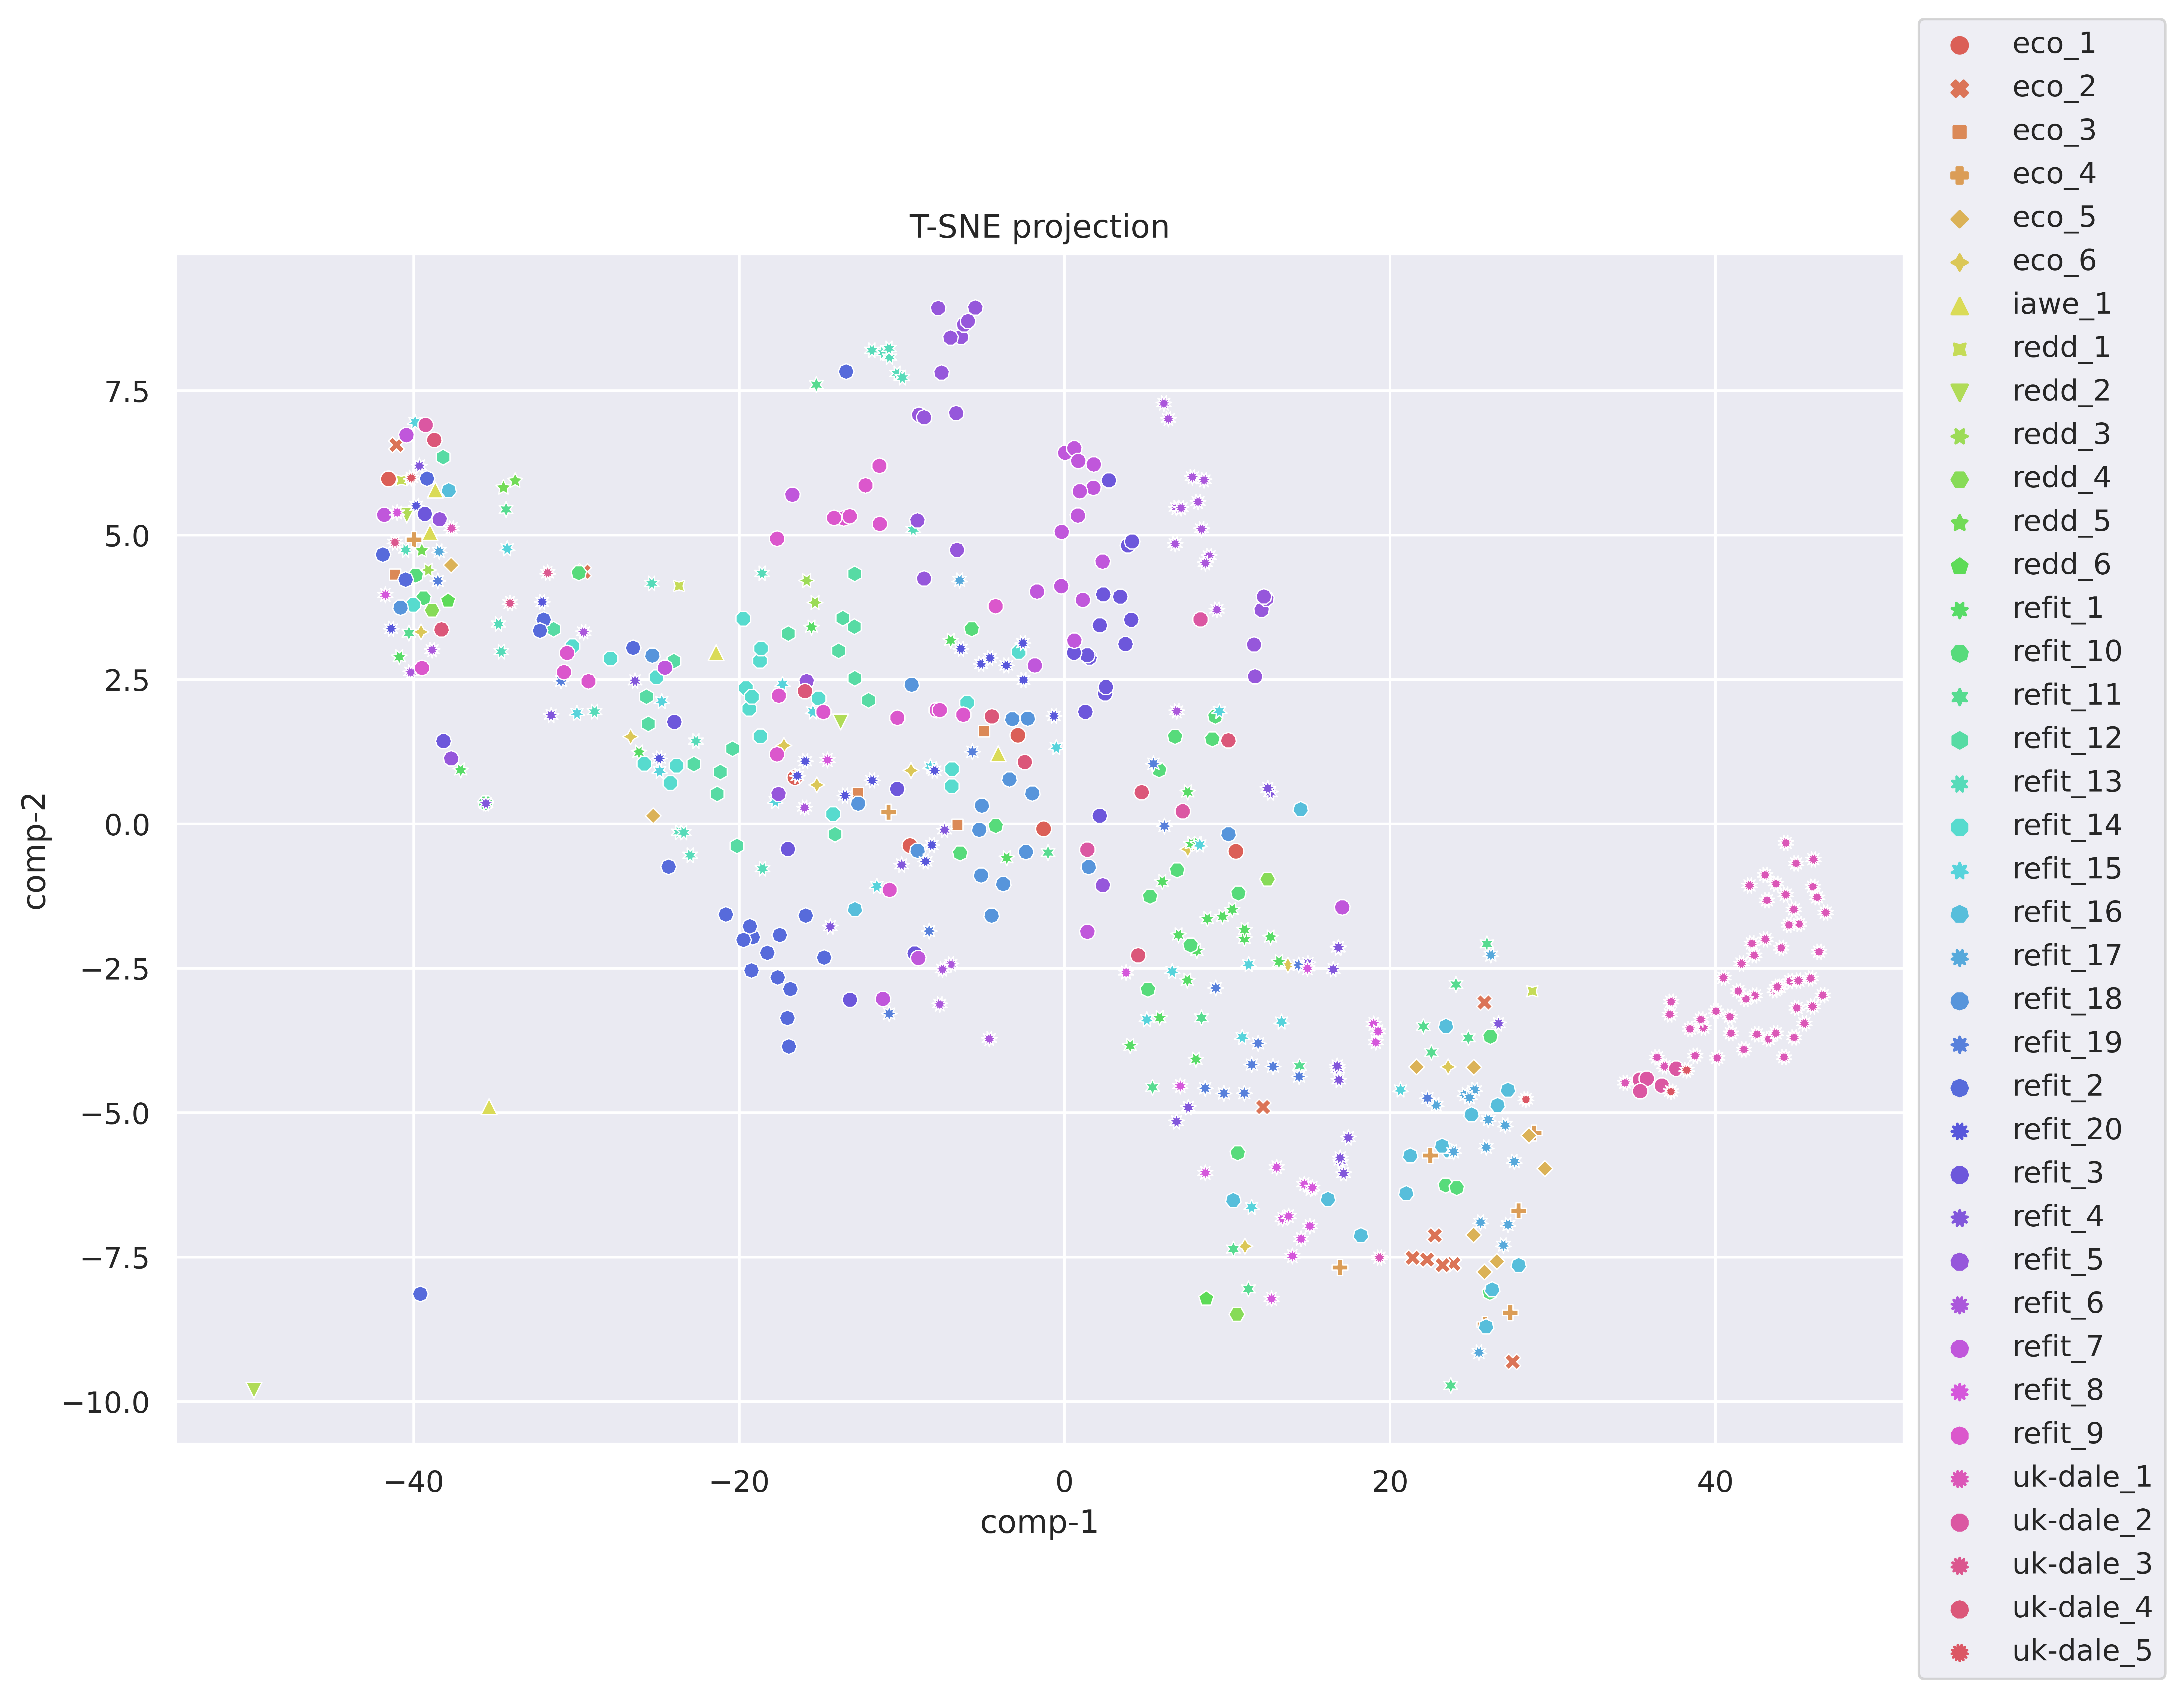
\includegraphics[width=1.2\textwidth]{Figures/TSNE/TSNE_per_building/non_norm/scatter_non_norm_all.png}
	\label{fig:tsne_scatter_non_norm_all}
\end{figure}

The figure \ref{fig:tsne_pb_img_scatter_allall} presents the actual load profile,
behind each sample. It is possible to see that on the left there are mostly samples 
with very little activity, and on the left, we see samples with more activity.
Since the two plotted components are of a higher dimension, it is hard to 
guess what they describe in our words. 
As said t-SNE gives us the intuition how load profiles are connected in higher-dimensional space.

\begin{figure}[H]
	\centering
	\caption{"Per building data for all buildings images"}
	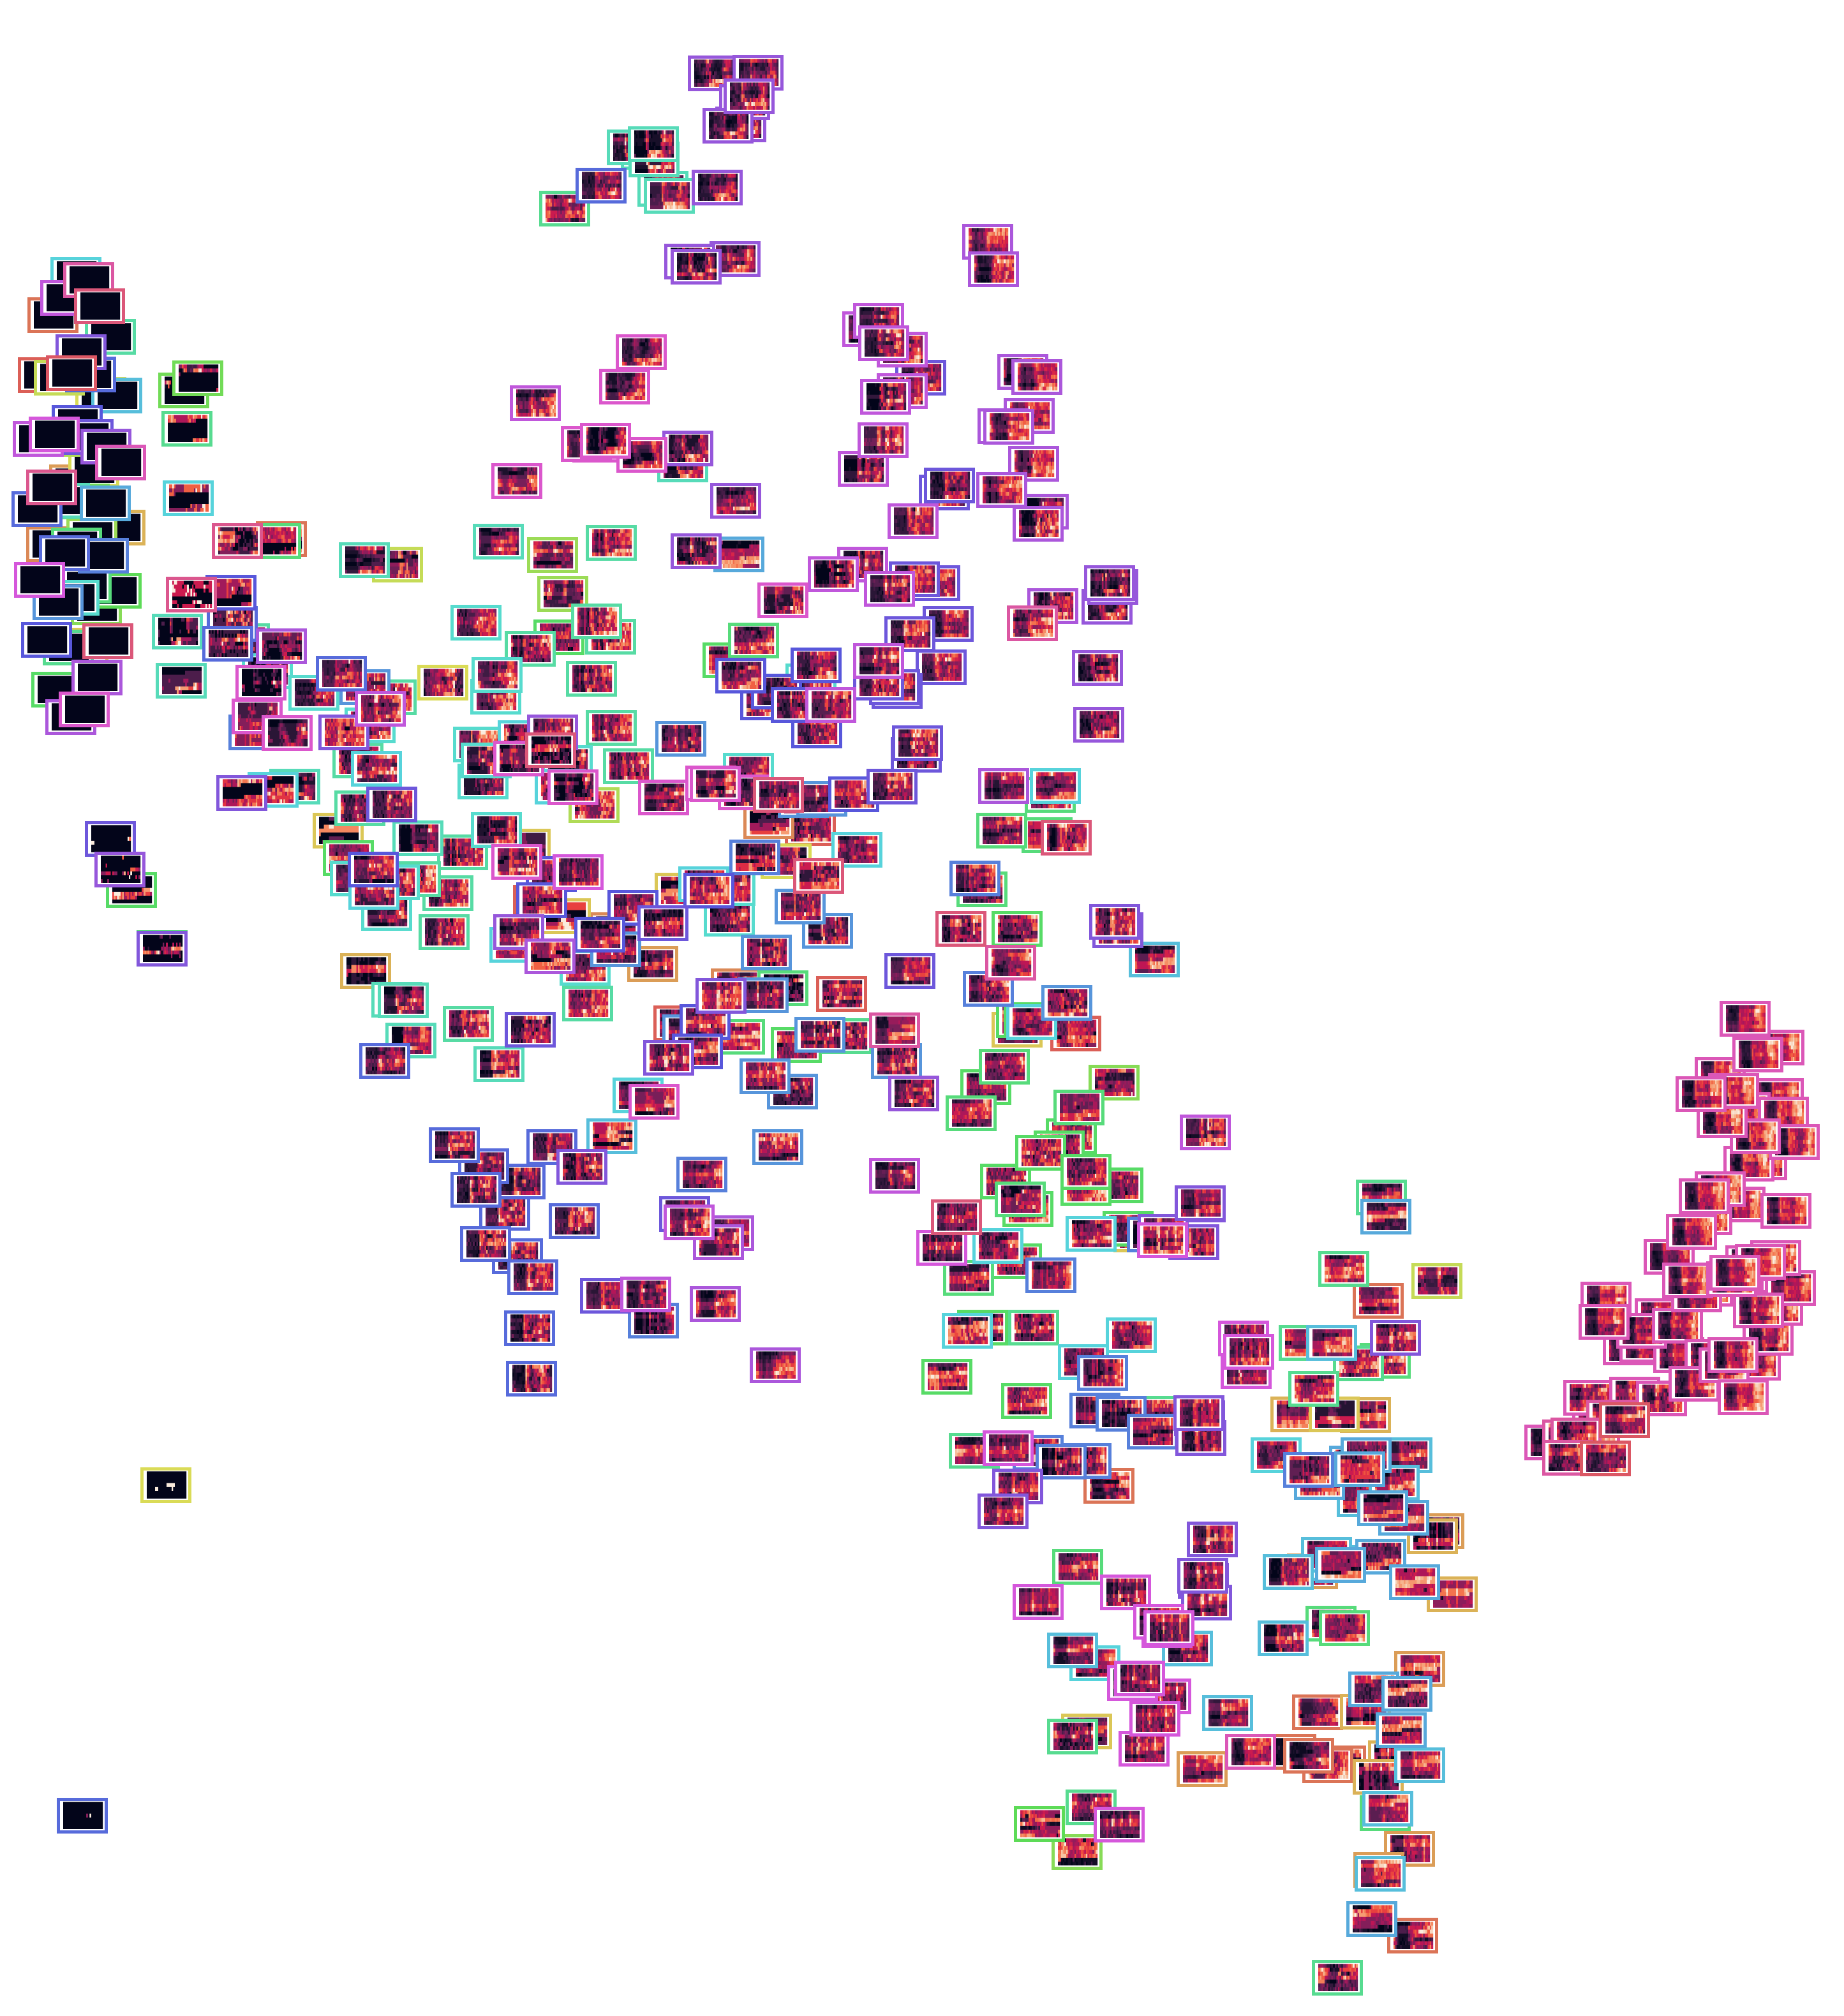
\includegraphics[width=.9\textwidth]{Figures/TSNE/TSNE_per_building/non_norm/img_scatter_allall.png}
	\label{fig:tsne_pb_img_scatter_allall}
\end{figure}

\subsubsection{Normalise samples}

To solve the issue mentioned we have to normalize the data between 0 and 1.
The figure \ref{fig:tsne_pb_scatter_all_all} shows how normalizing samples affect the algorithm.
The samples are much closer to each other, while it is still possible to see the individual clusters.

\begin{figure}[H]
	\centering
	\caption{"Per building data for all buildings"}
	\includegraphics[width=1.2\textwidth]{Figures/TSNE/TSNE_per_building/all/scatter_all_all.png}
	\label{fig:tsne_pb_scatter_all_all}
\end{figure}

The figure \ref{fig:tsne_pb_img_norm_scatter_allall} presents only the main cluster 
of samples, since the smaller cluster presents mostly low entropy data. It can be seen on 
far left on figure \ref{fig:tsne_pb_img_scatter_allall}, all trough the shape of cluster is 
oval, they present blank load profiles.
\begin{figure}[H]
	\centering
	\caption{"Per building data for refit buildings images"}
	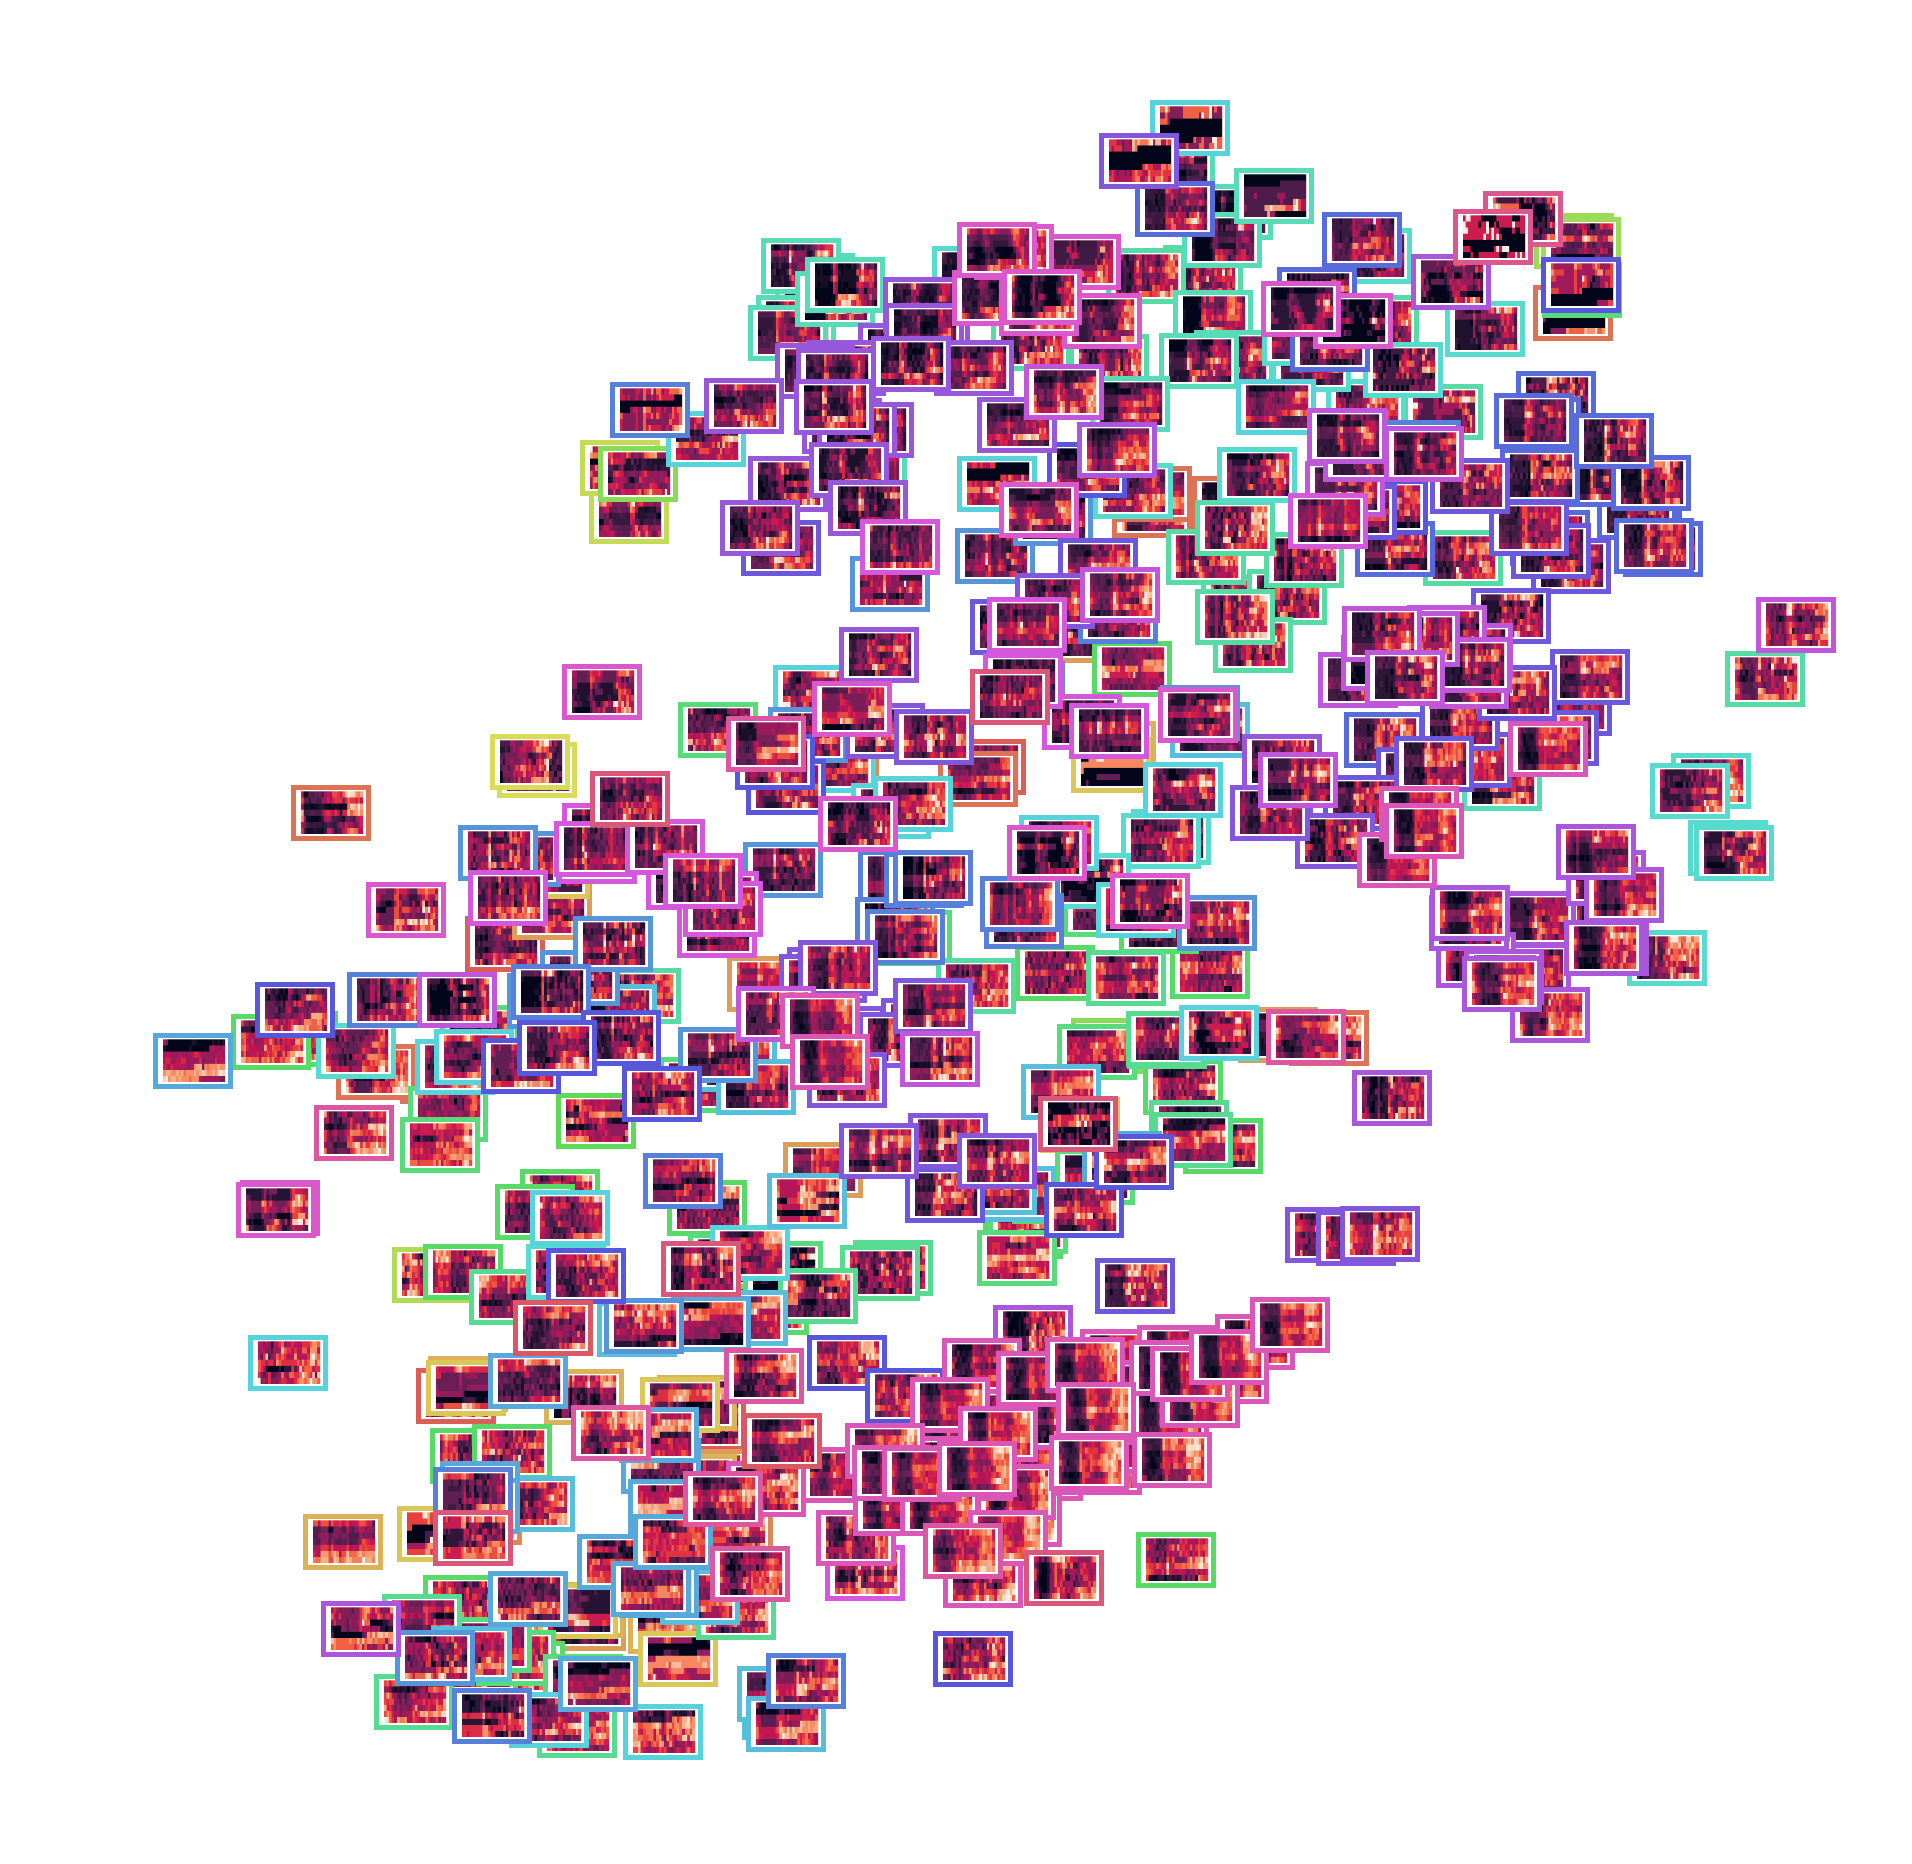
\includegraphics[width=.9\textwidth]{Figures/TSNE/TSNE_per_building/all/img_scatter_allall.png}
	\label{fig:tsne_pb_img_norm_scatter_allall}
\end{figure}

\subsection{Per-appliance}

Per-appliance allows us to focus on each appliance separately.
By changing the labels and data we can again analyze different things.

\subsubsection{Single appliance over many buildings}

Using only one appliance and using the building as a label,
allows us to examine how the same type of appliance is being used across different buildings.

% \subsubsubsection{fridge, freezers and fridge freezers}
Fridges are generally interesting when it comes to user behavior, since the user does not affect
its operation apart from opening the door and turning on the light inside. Usualy this
event is dwarfed by a number of activations of a compressor. All this also means that
That the usage should be generally the across all buildings. 
This can be seen on figure \ref{fig:tsne_pa_scatter_all_fridge},
where, apart from REFIT building 1 and 11, there are no clusters.

\begin{figure}[H]
	\centering
	\caption{"Per appliance data for all buildings"}
	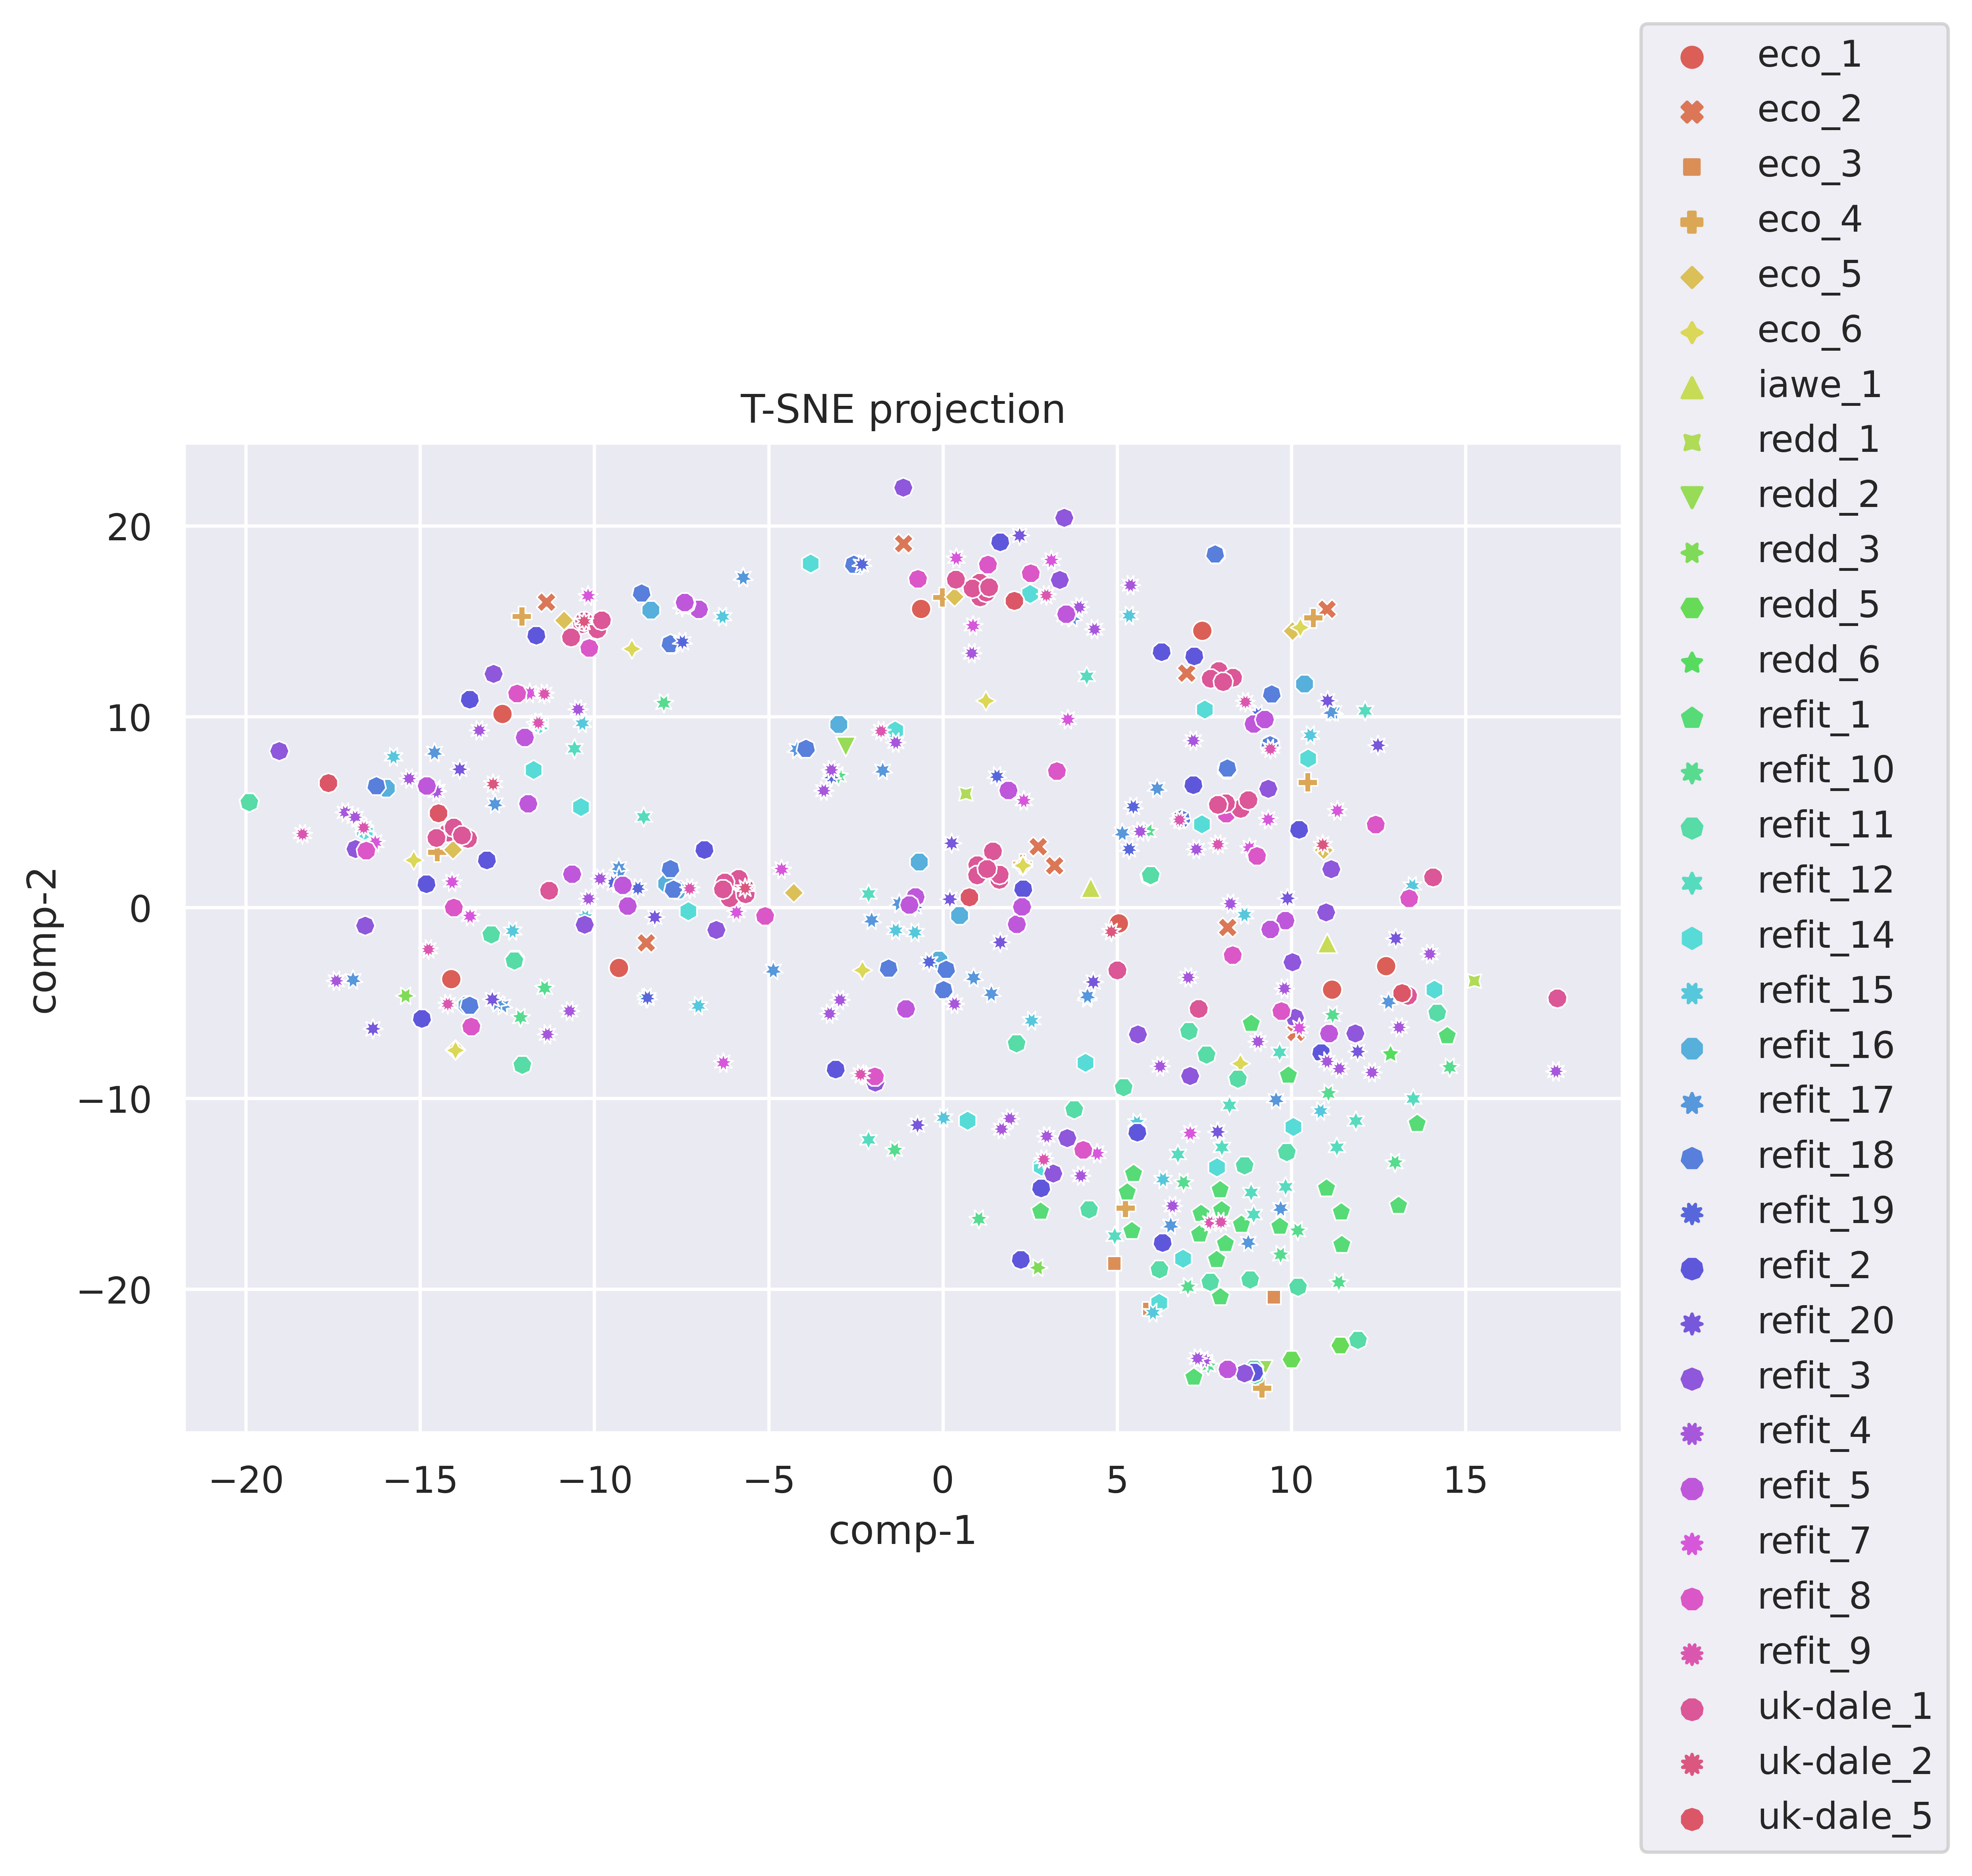
\includegraphics[width=1.2\textwidth]{Figures/TSNE/TSNE_per_appliance/all/scatter_all_fridge_freeezer_fridge freezer.png}
	\label{fig:tsne_pa_scatter_all_fridge}
\end{figure}

\ref{fig:tsne_pa_img_scatter_all_fridge} Shows mostly bright images, apart from few outliers.
Load profiles scattered in a circle are generaly less dynamic than the ones in the bottom.

\begin{figure}[H]
	\centering
	\caption{"Per appliance data for refit buildings images"}
	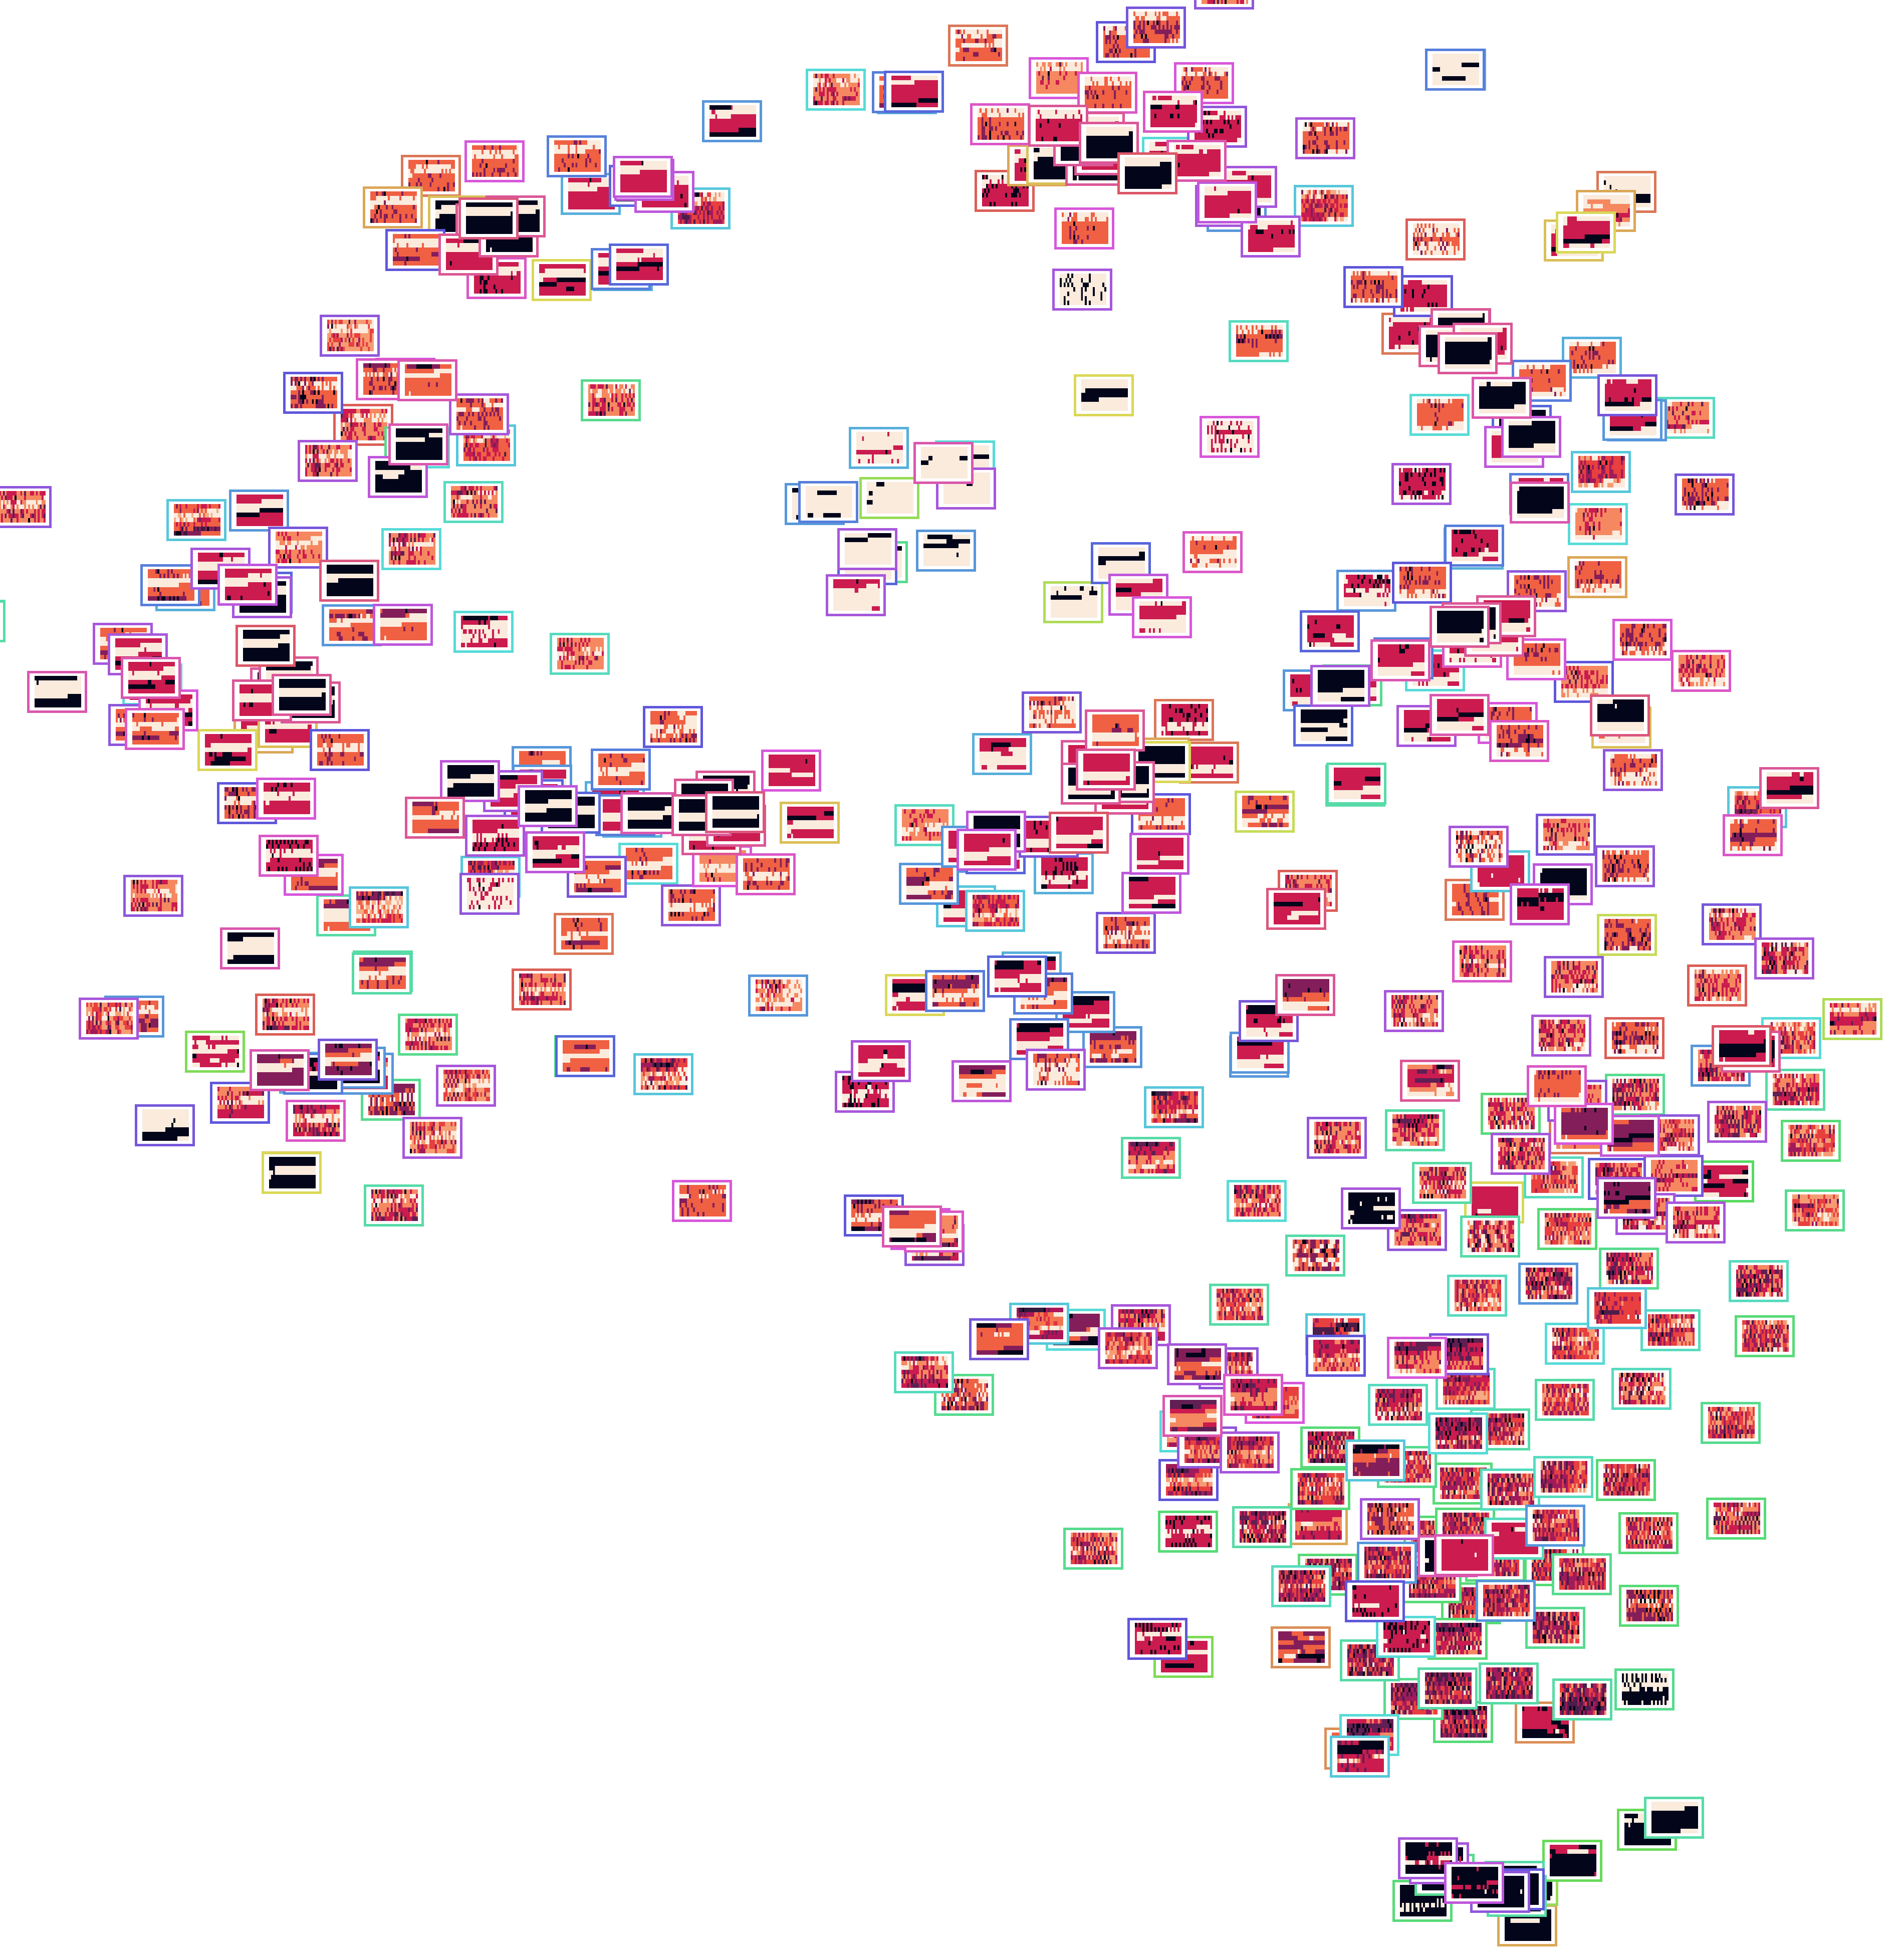
\includegraphics[width=.9\textwidth]{Figures/TSNE/TSNE_per_appliance/all/img_scatter_allfridge_freeezer_fridge freezer.png}
	\label{fig:tsne_pa_img_scatter_all_fridge}
\end{figure}


% \subsubsubsection{kettle}
Compared to fridges, kettles have much more clear clusters, that are spaced out 
between each other. This could mean that every household uses a kettle a bit differently. 
This cluster is a good example where we can see how strong is a routine of a user,
The closer together the clusters, the higher is the routine since samples have to be 
close to each other.

\begin{figure}[H]
	\centering
	\caption{"Per appliance data for all buildings"}
	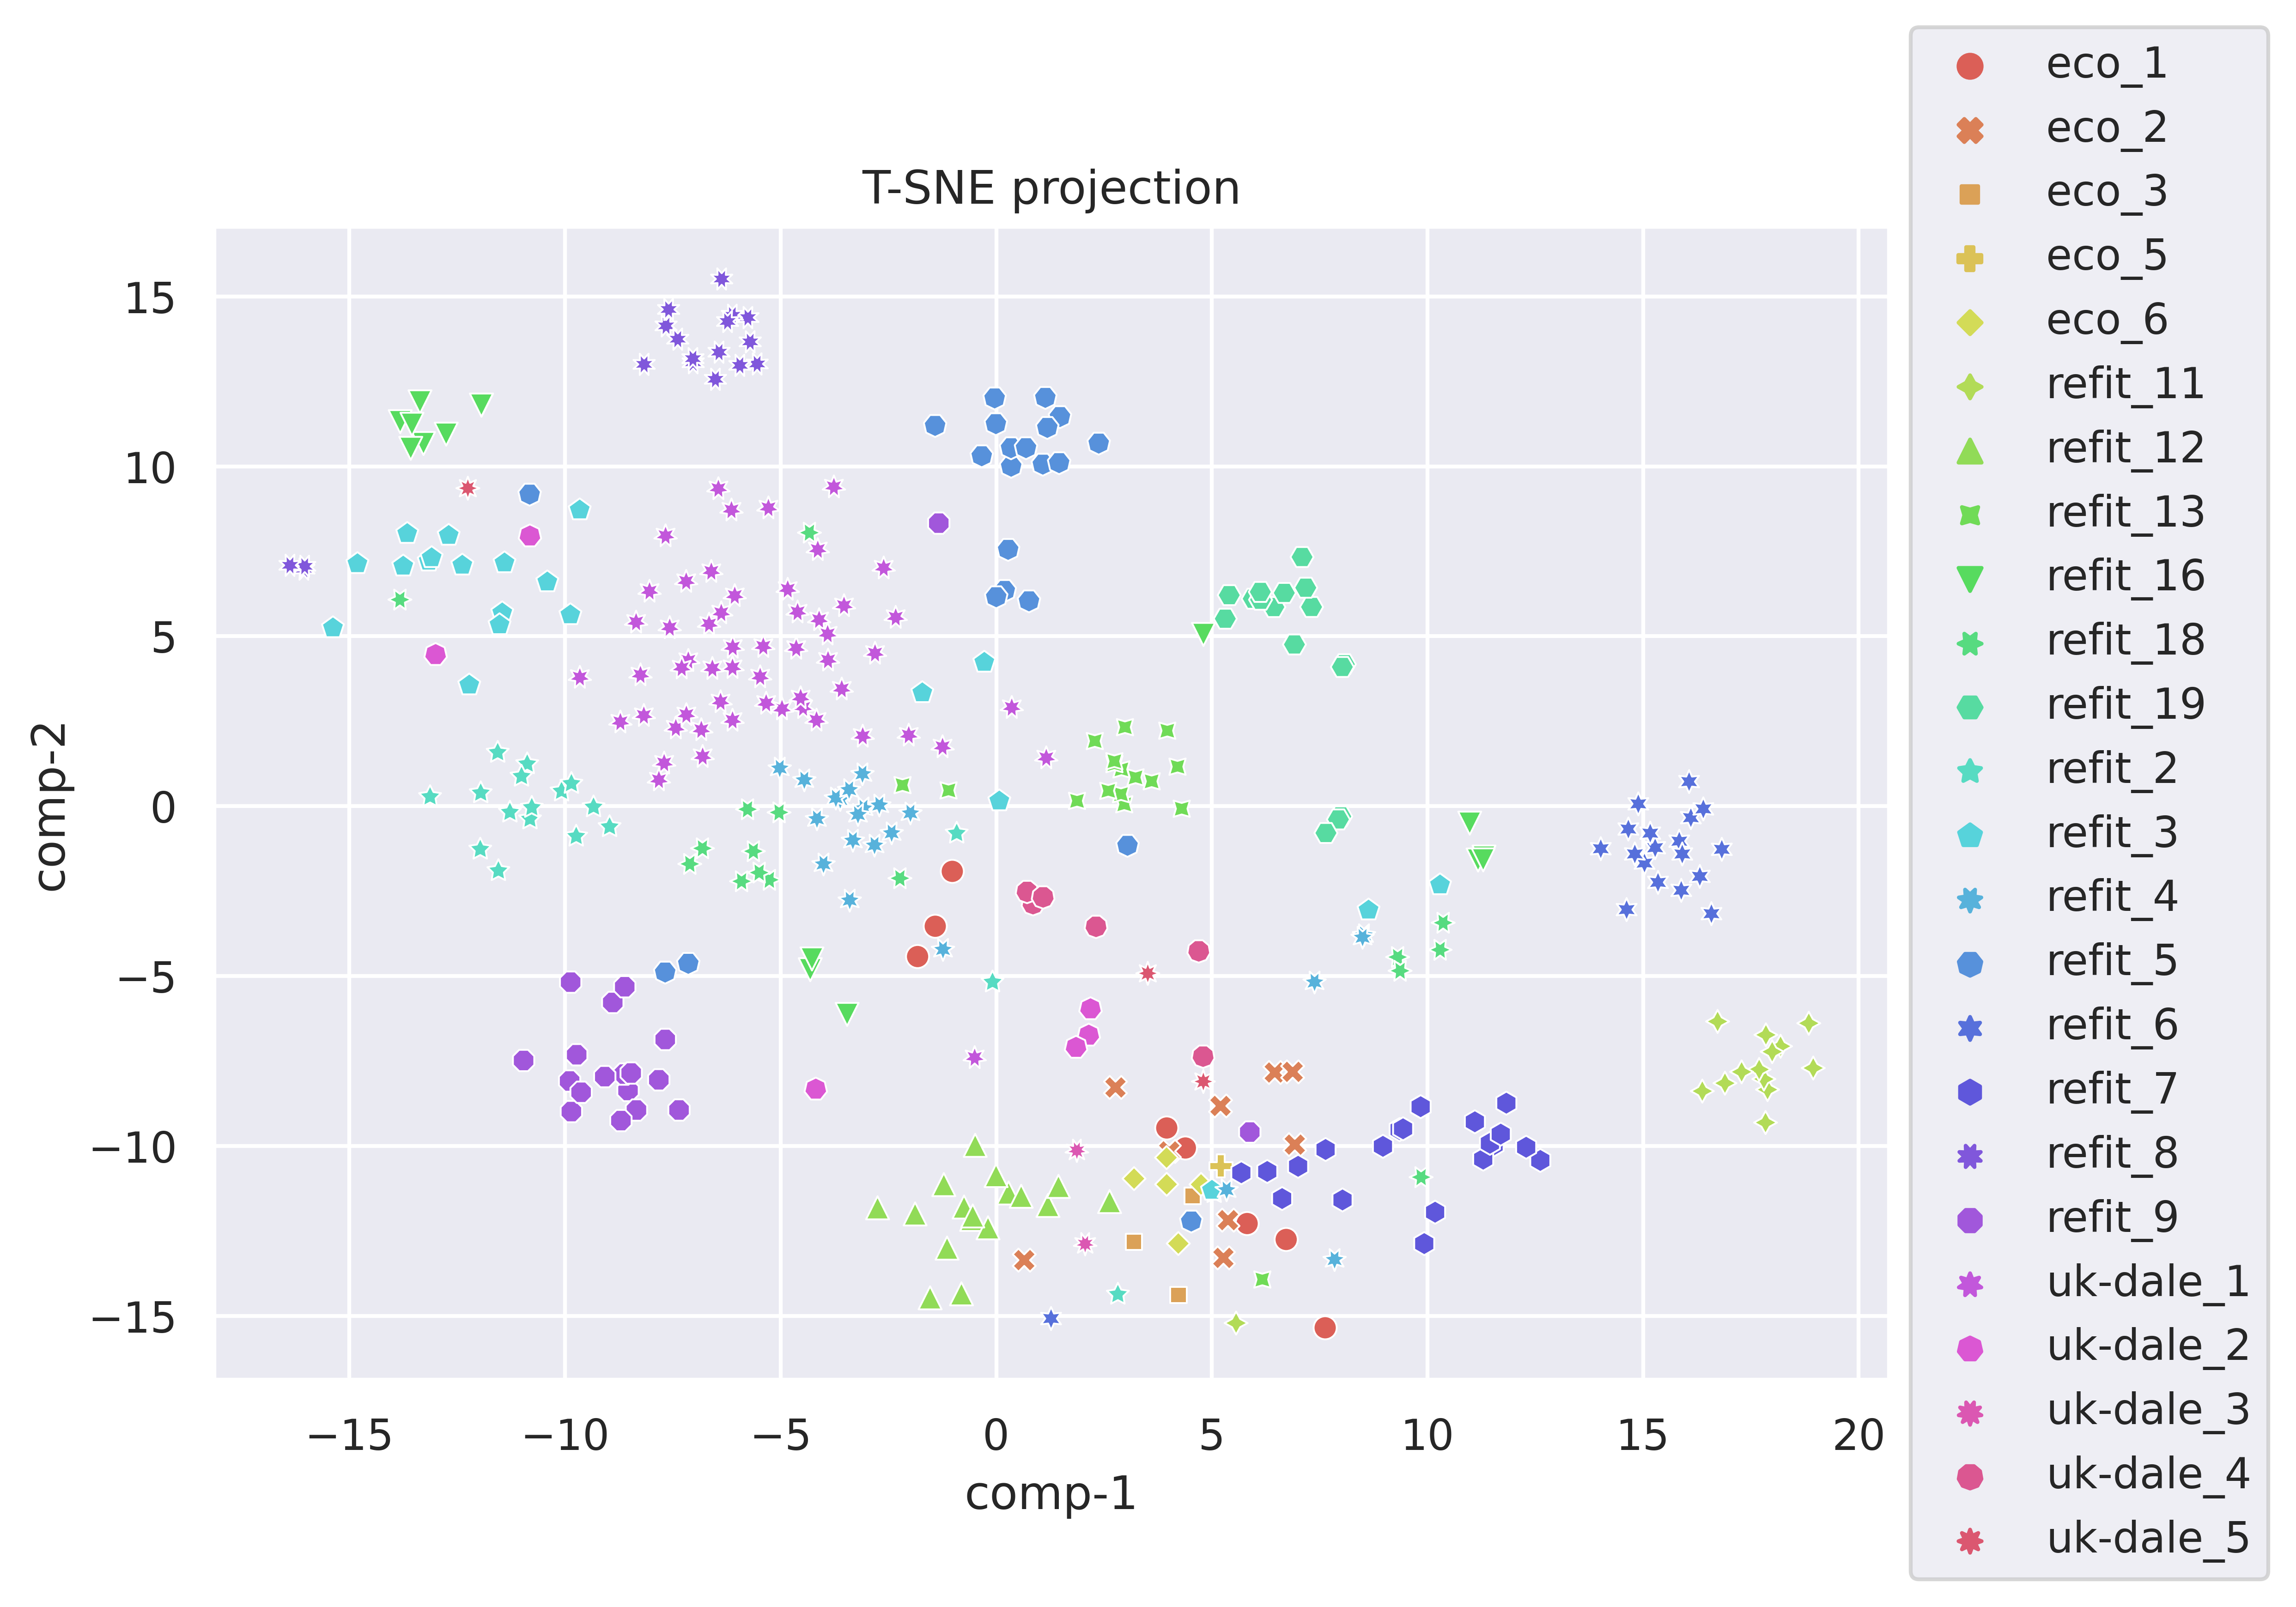
\includegraphics[width=1.2\textwidth]{Figures/TSNE/TSNE_per_appliance/all/scatter_all_kettle.png}
	\label{fig:tsne_pa_scatter_all_kettle}
\end{figure}

The figure \ref{fig:tsne_pa_img_scatter_all_kettle} show us that images on the lower part 
of the plot contain less activity than the others.

\begin{figure}[H]
	\centering
	\caption{"Per appliance data for refit buildings images"}
	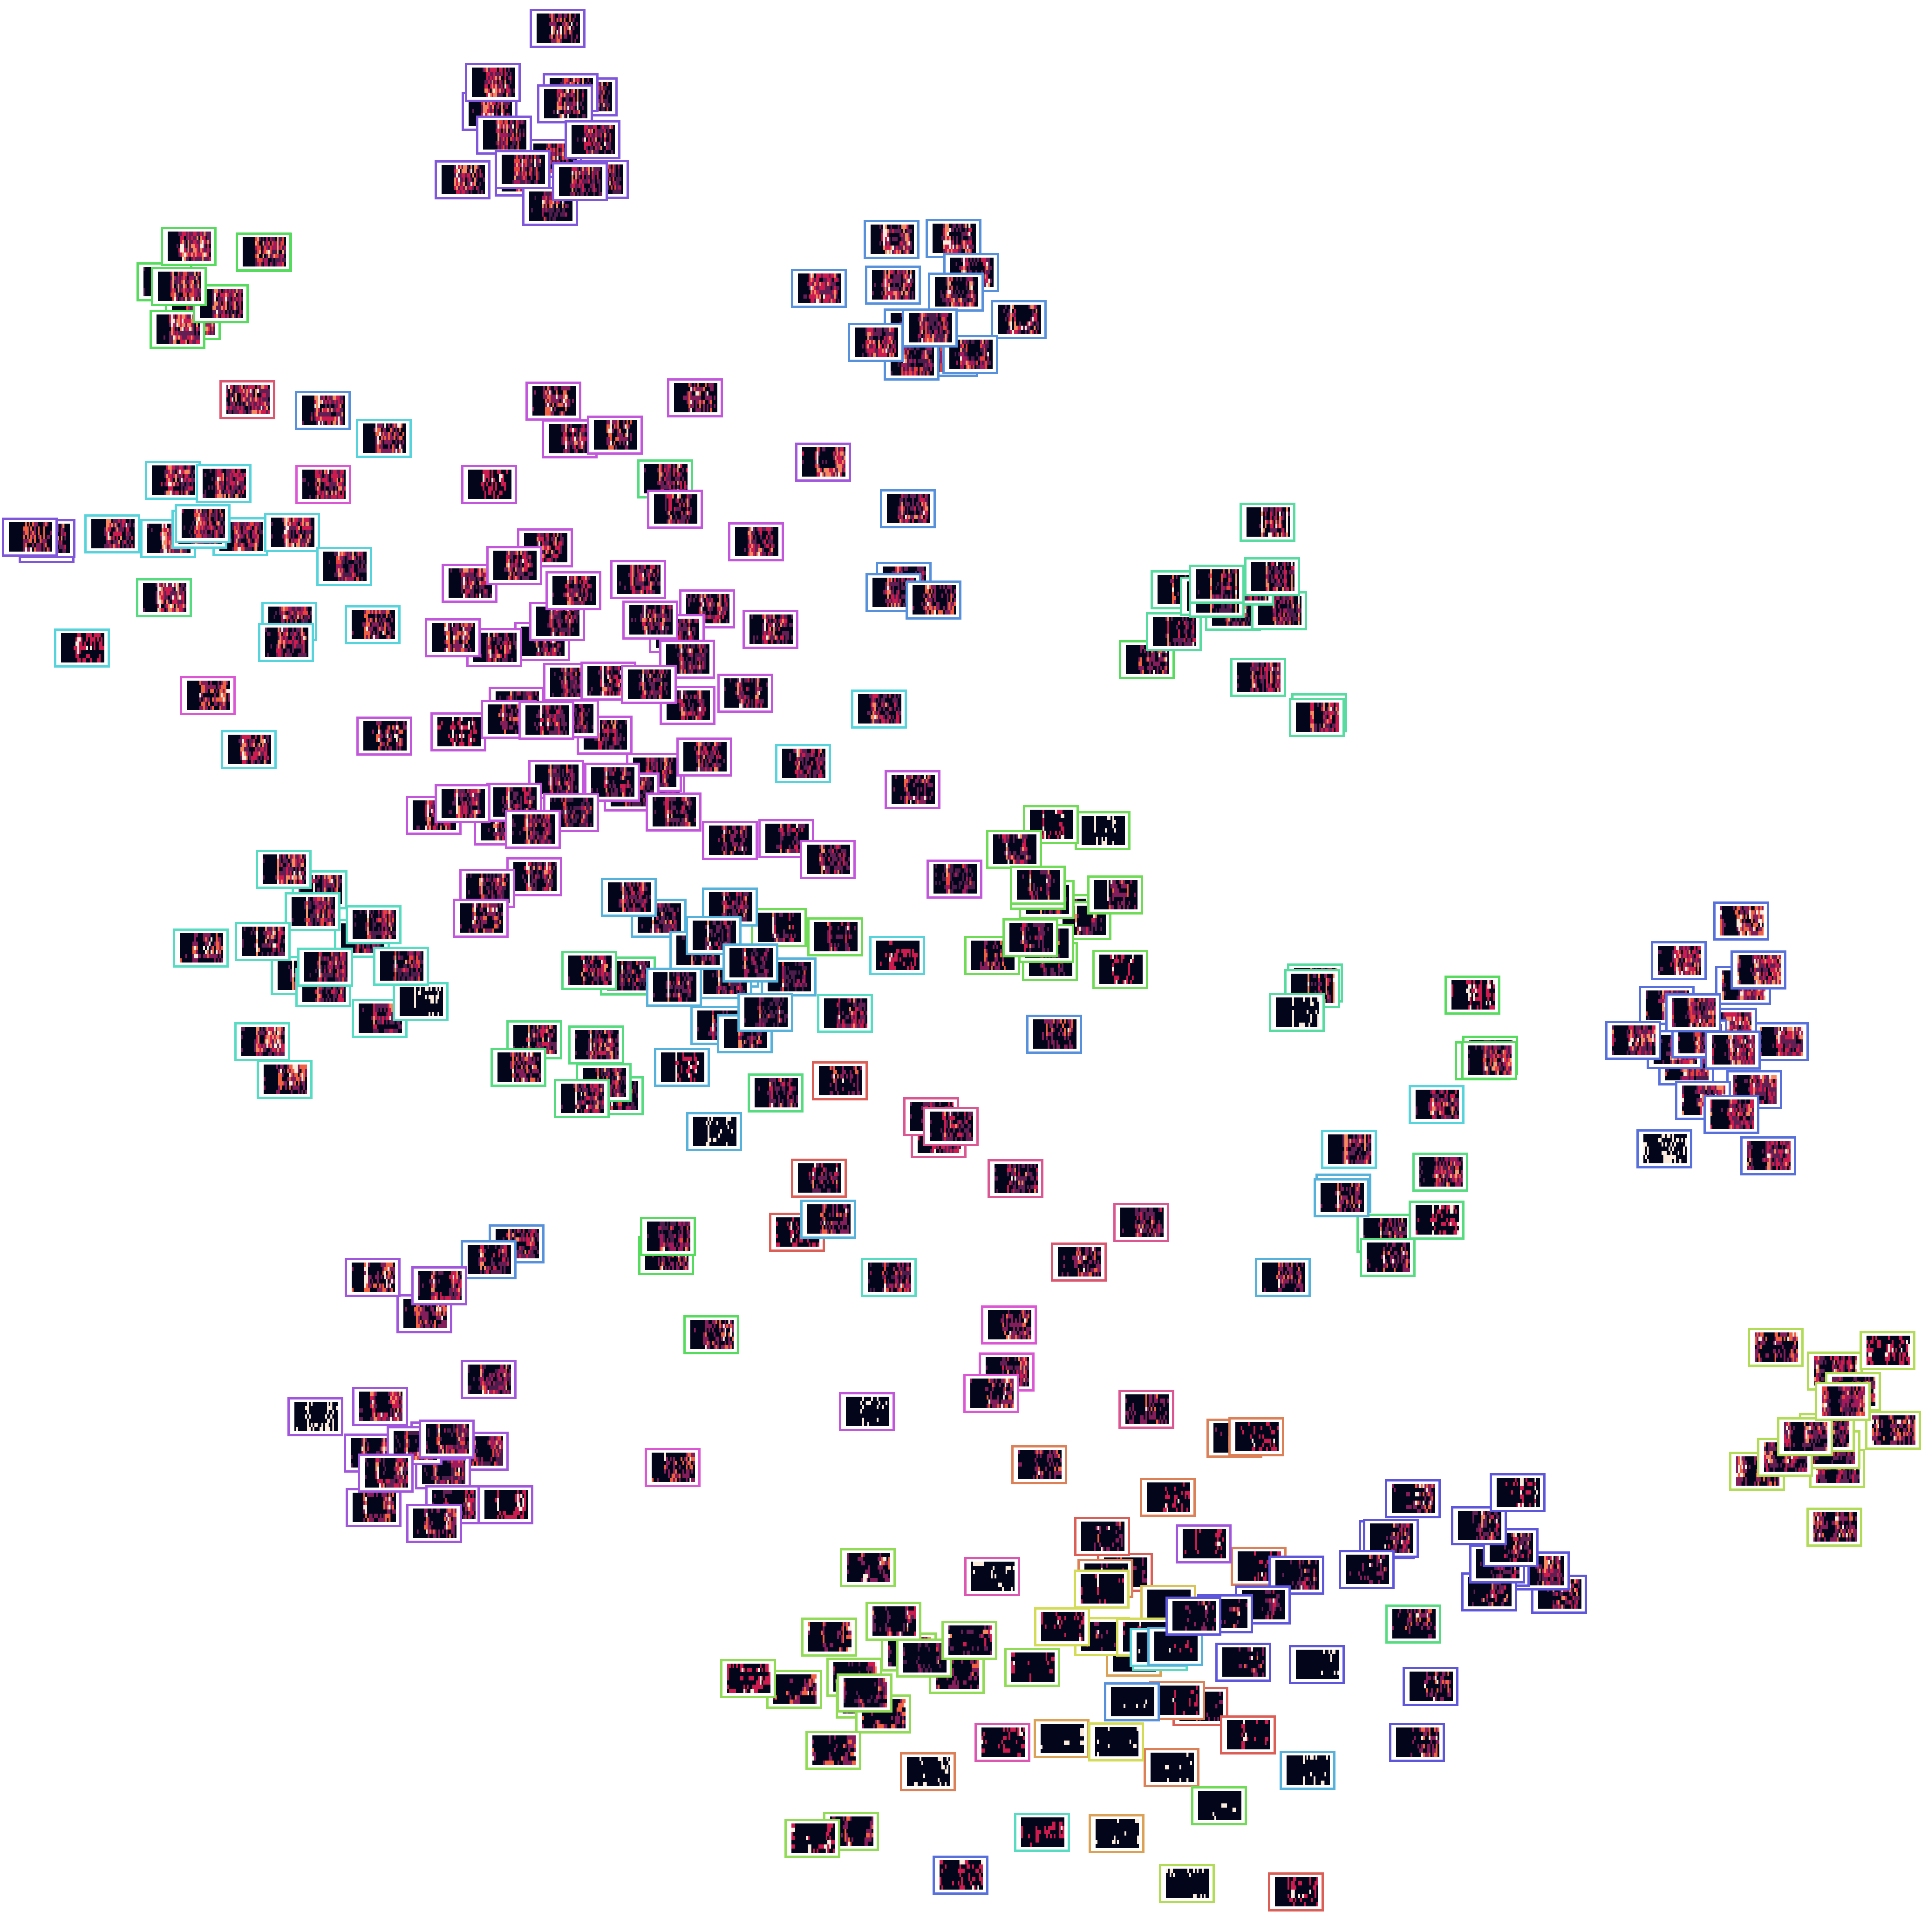
\includegraphics[width=.9\textwidth]{Figures/TSNE/TSNE_per_appliance/all/img_scatter_allkettle.png}
	\label{fig:tsne_pa_img_scatter_all_kettle}
\end{figure}

% \subsubsubsection{microwave}
microwaves are again a bit different that the kettle. All trough the are more 
clustered than the fridges, they are less than the kettles, al trough 
they are generally used in a similar manor.
This could be due to additional electronics such as a clock are built into,
the applaince, this could lead to some samples being regired as turned on due to 
"dark" current. 

\begin{figure}[H]
	\centering
	\caption{"Per appliance data for all buildings"}
	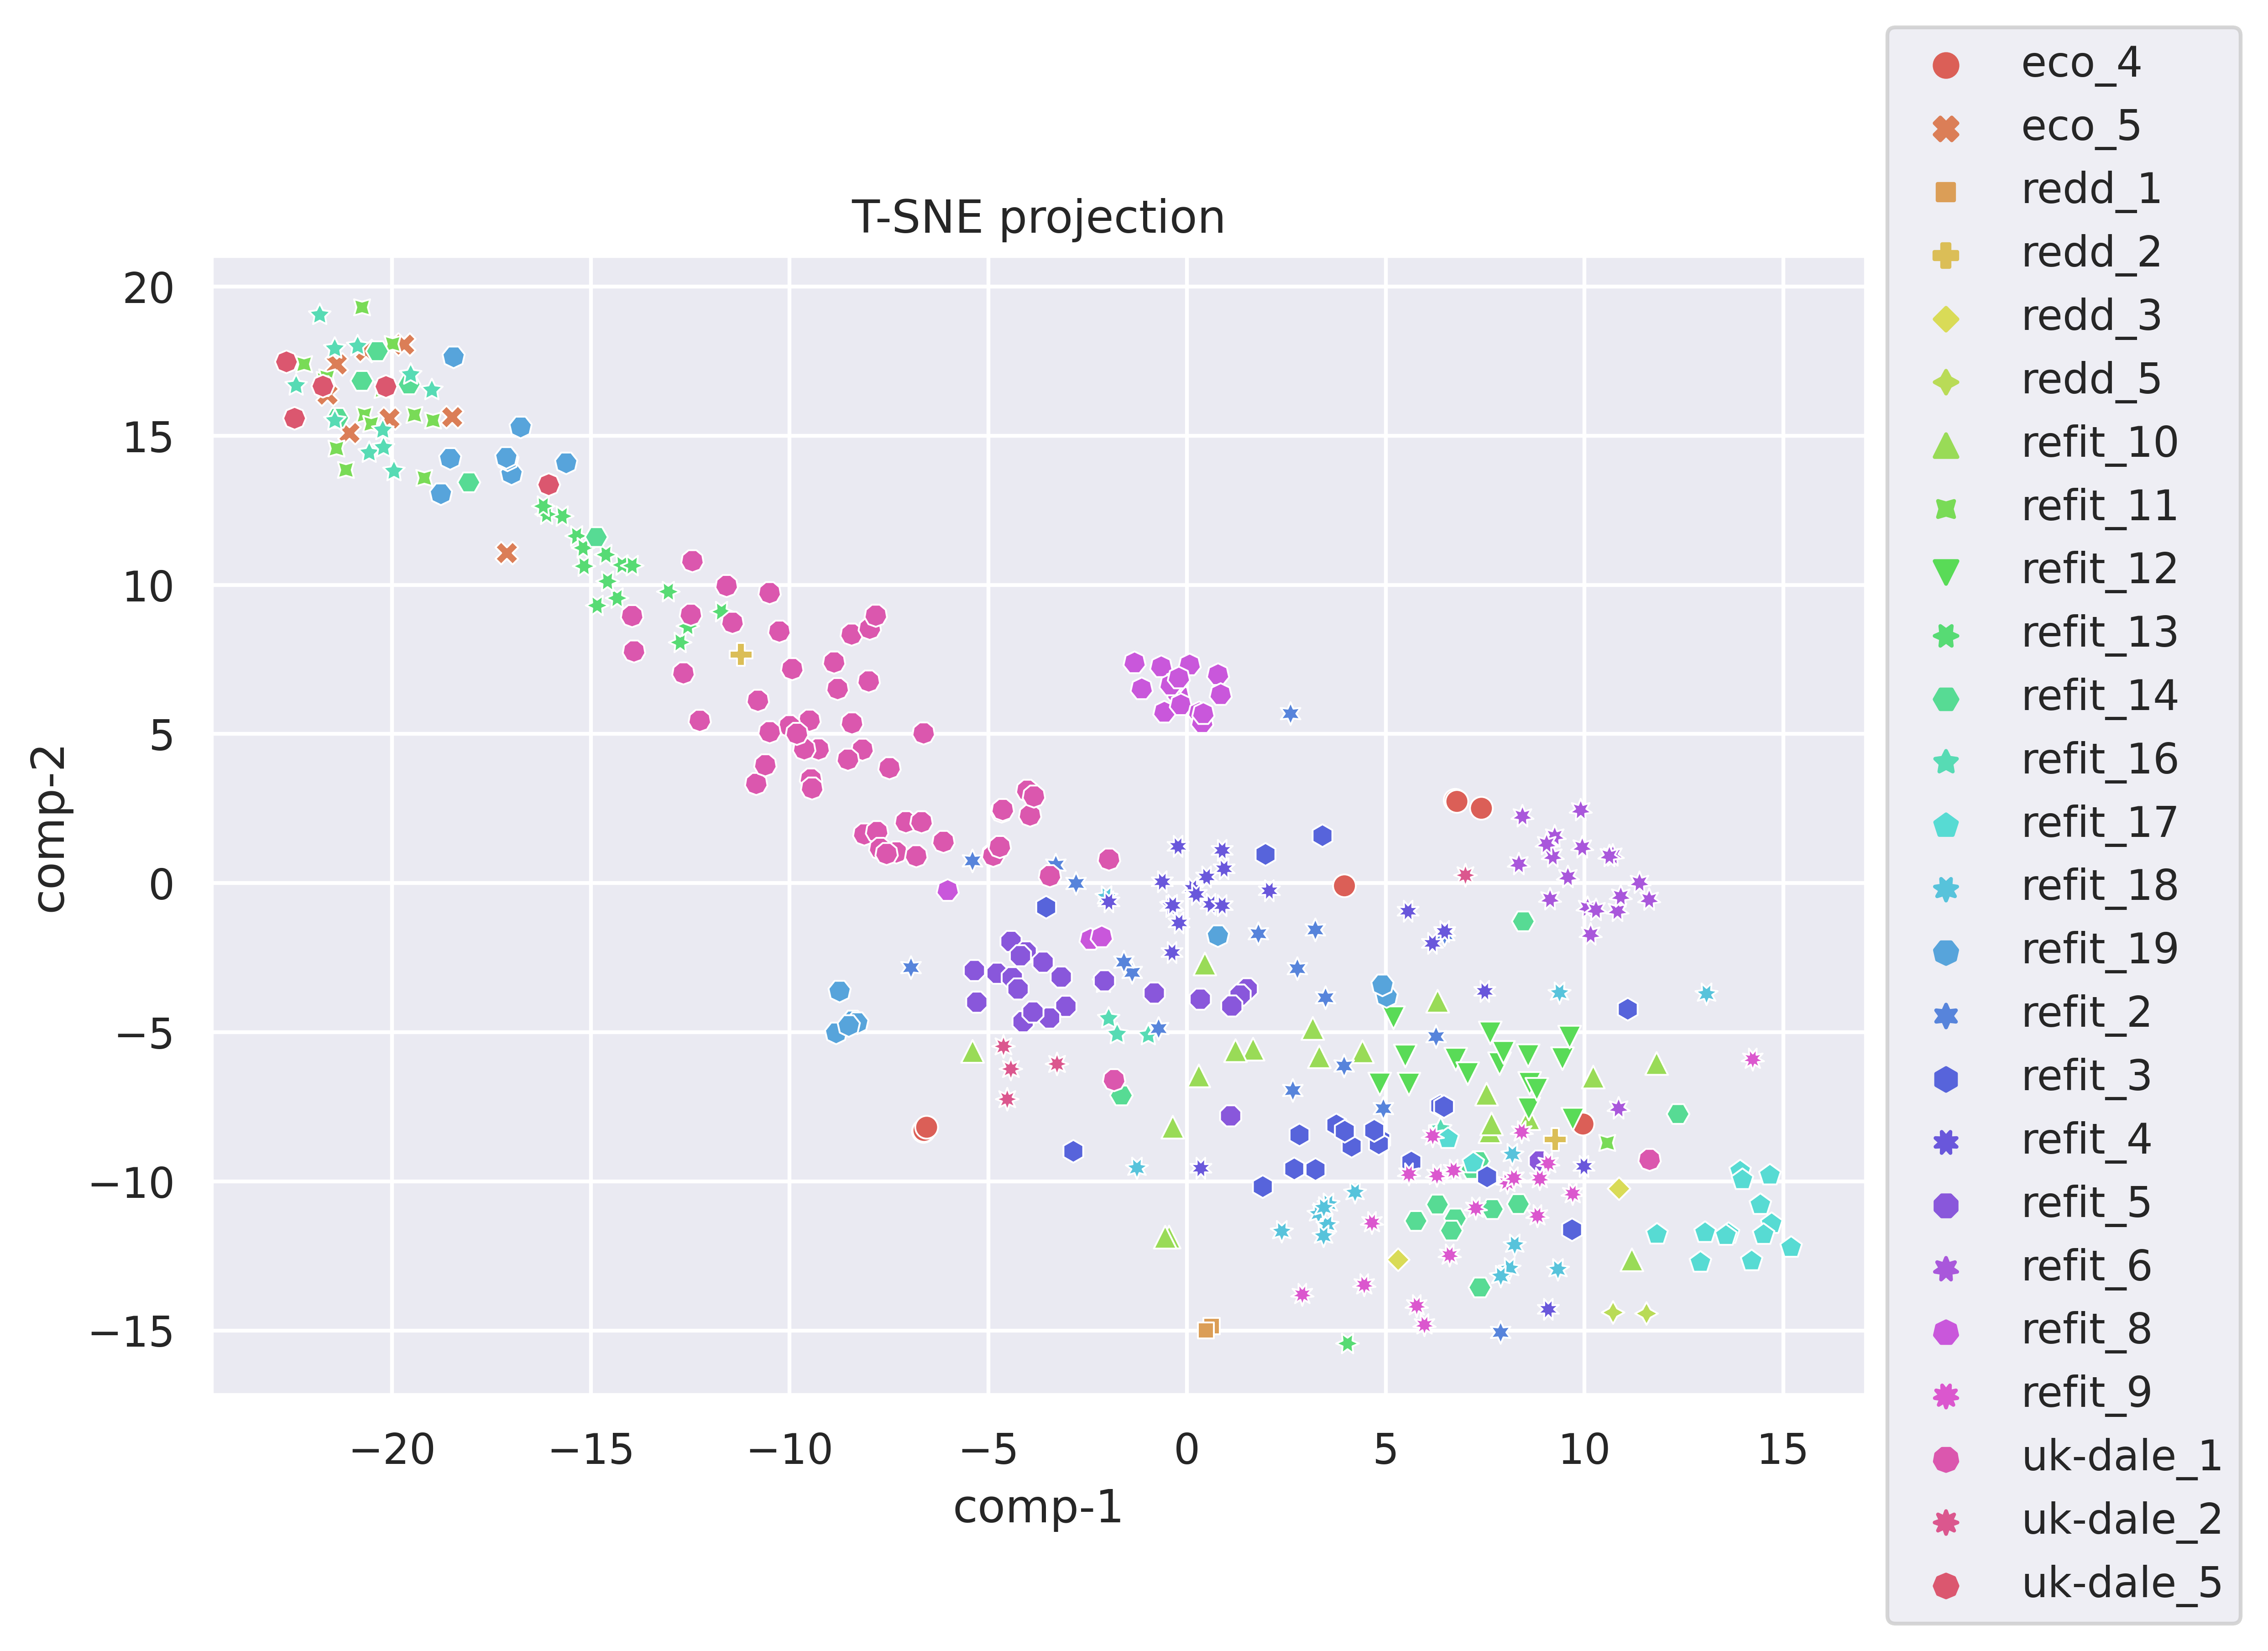
\includegraphics[width=1.2\textwidth]{Figures/TSNE/TSNE_per_appliance/all/scatter_all_microwave.png}
	\label{fig:tsne_pa_scatter_all_microwave}
\end{figure}

The false samples could be the ones in the upper left part of the plot, since they are bright.
Images at the other end show less lot less activity.

\begin{figure}[H]
	\centering
	\caption{"Per appliance data for refit buildings images"}
	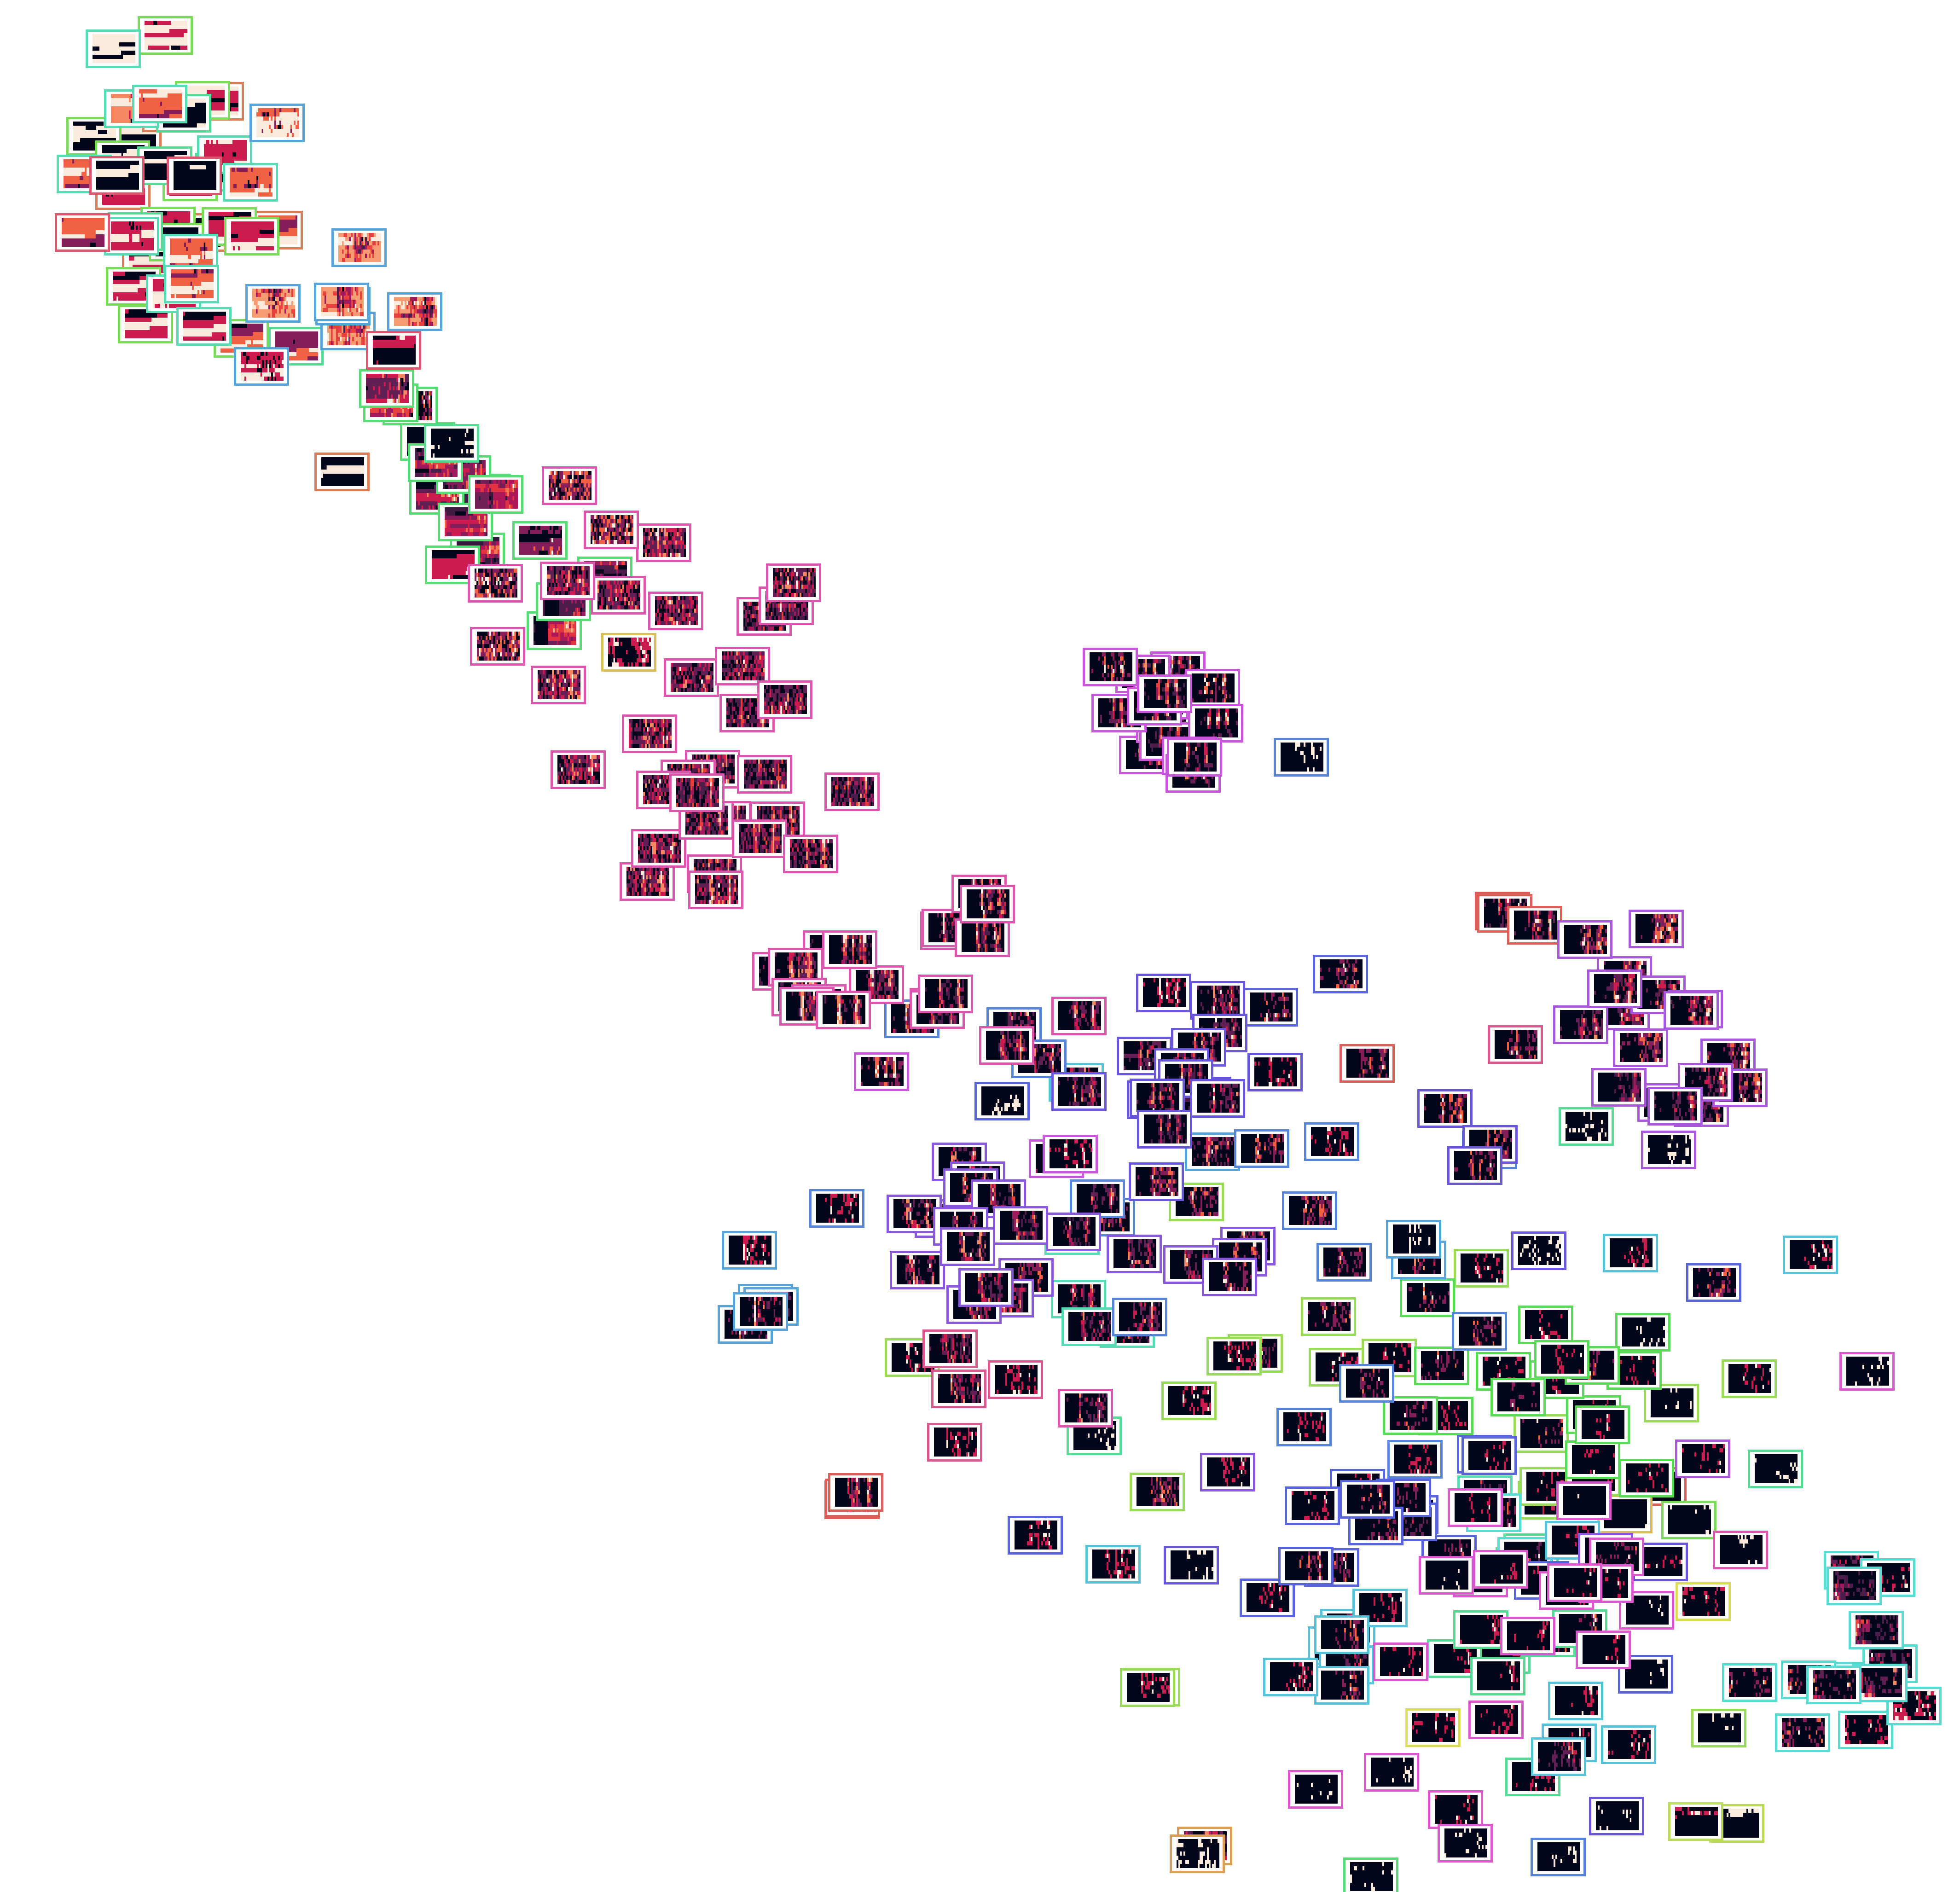
\includegraphics[width=.9\textwidth]{Figures/TSNE/TSNE_per_appliance/all/img_scatter_allmicrowave.png}
	\label{fig:tsne_pa_img_scatter_all_microwave}
\end{figure}

% \subsubsubsection{television}
The last examples are TV. They were chosen since they were common across all datasets.
Interestingly tvs also show genearly nicely form clusters where most of them are close 
together, with few outliers.
This could mean that most of the households used tv in a simialar way, with few examples.
The samples in some clusters are also close to each other, which could also indicate 
a higher routine.

\begin{figure}[H]
	\centering
	\caption{"Per appliance data for all buildings"}
	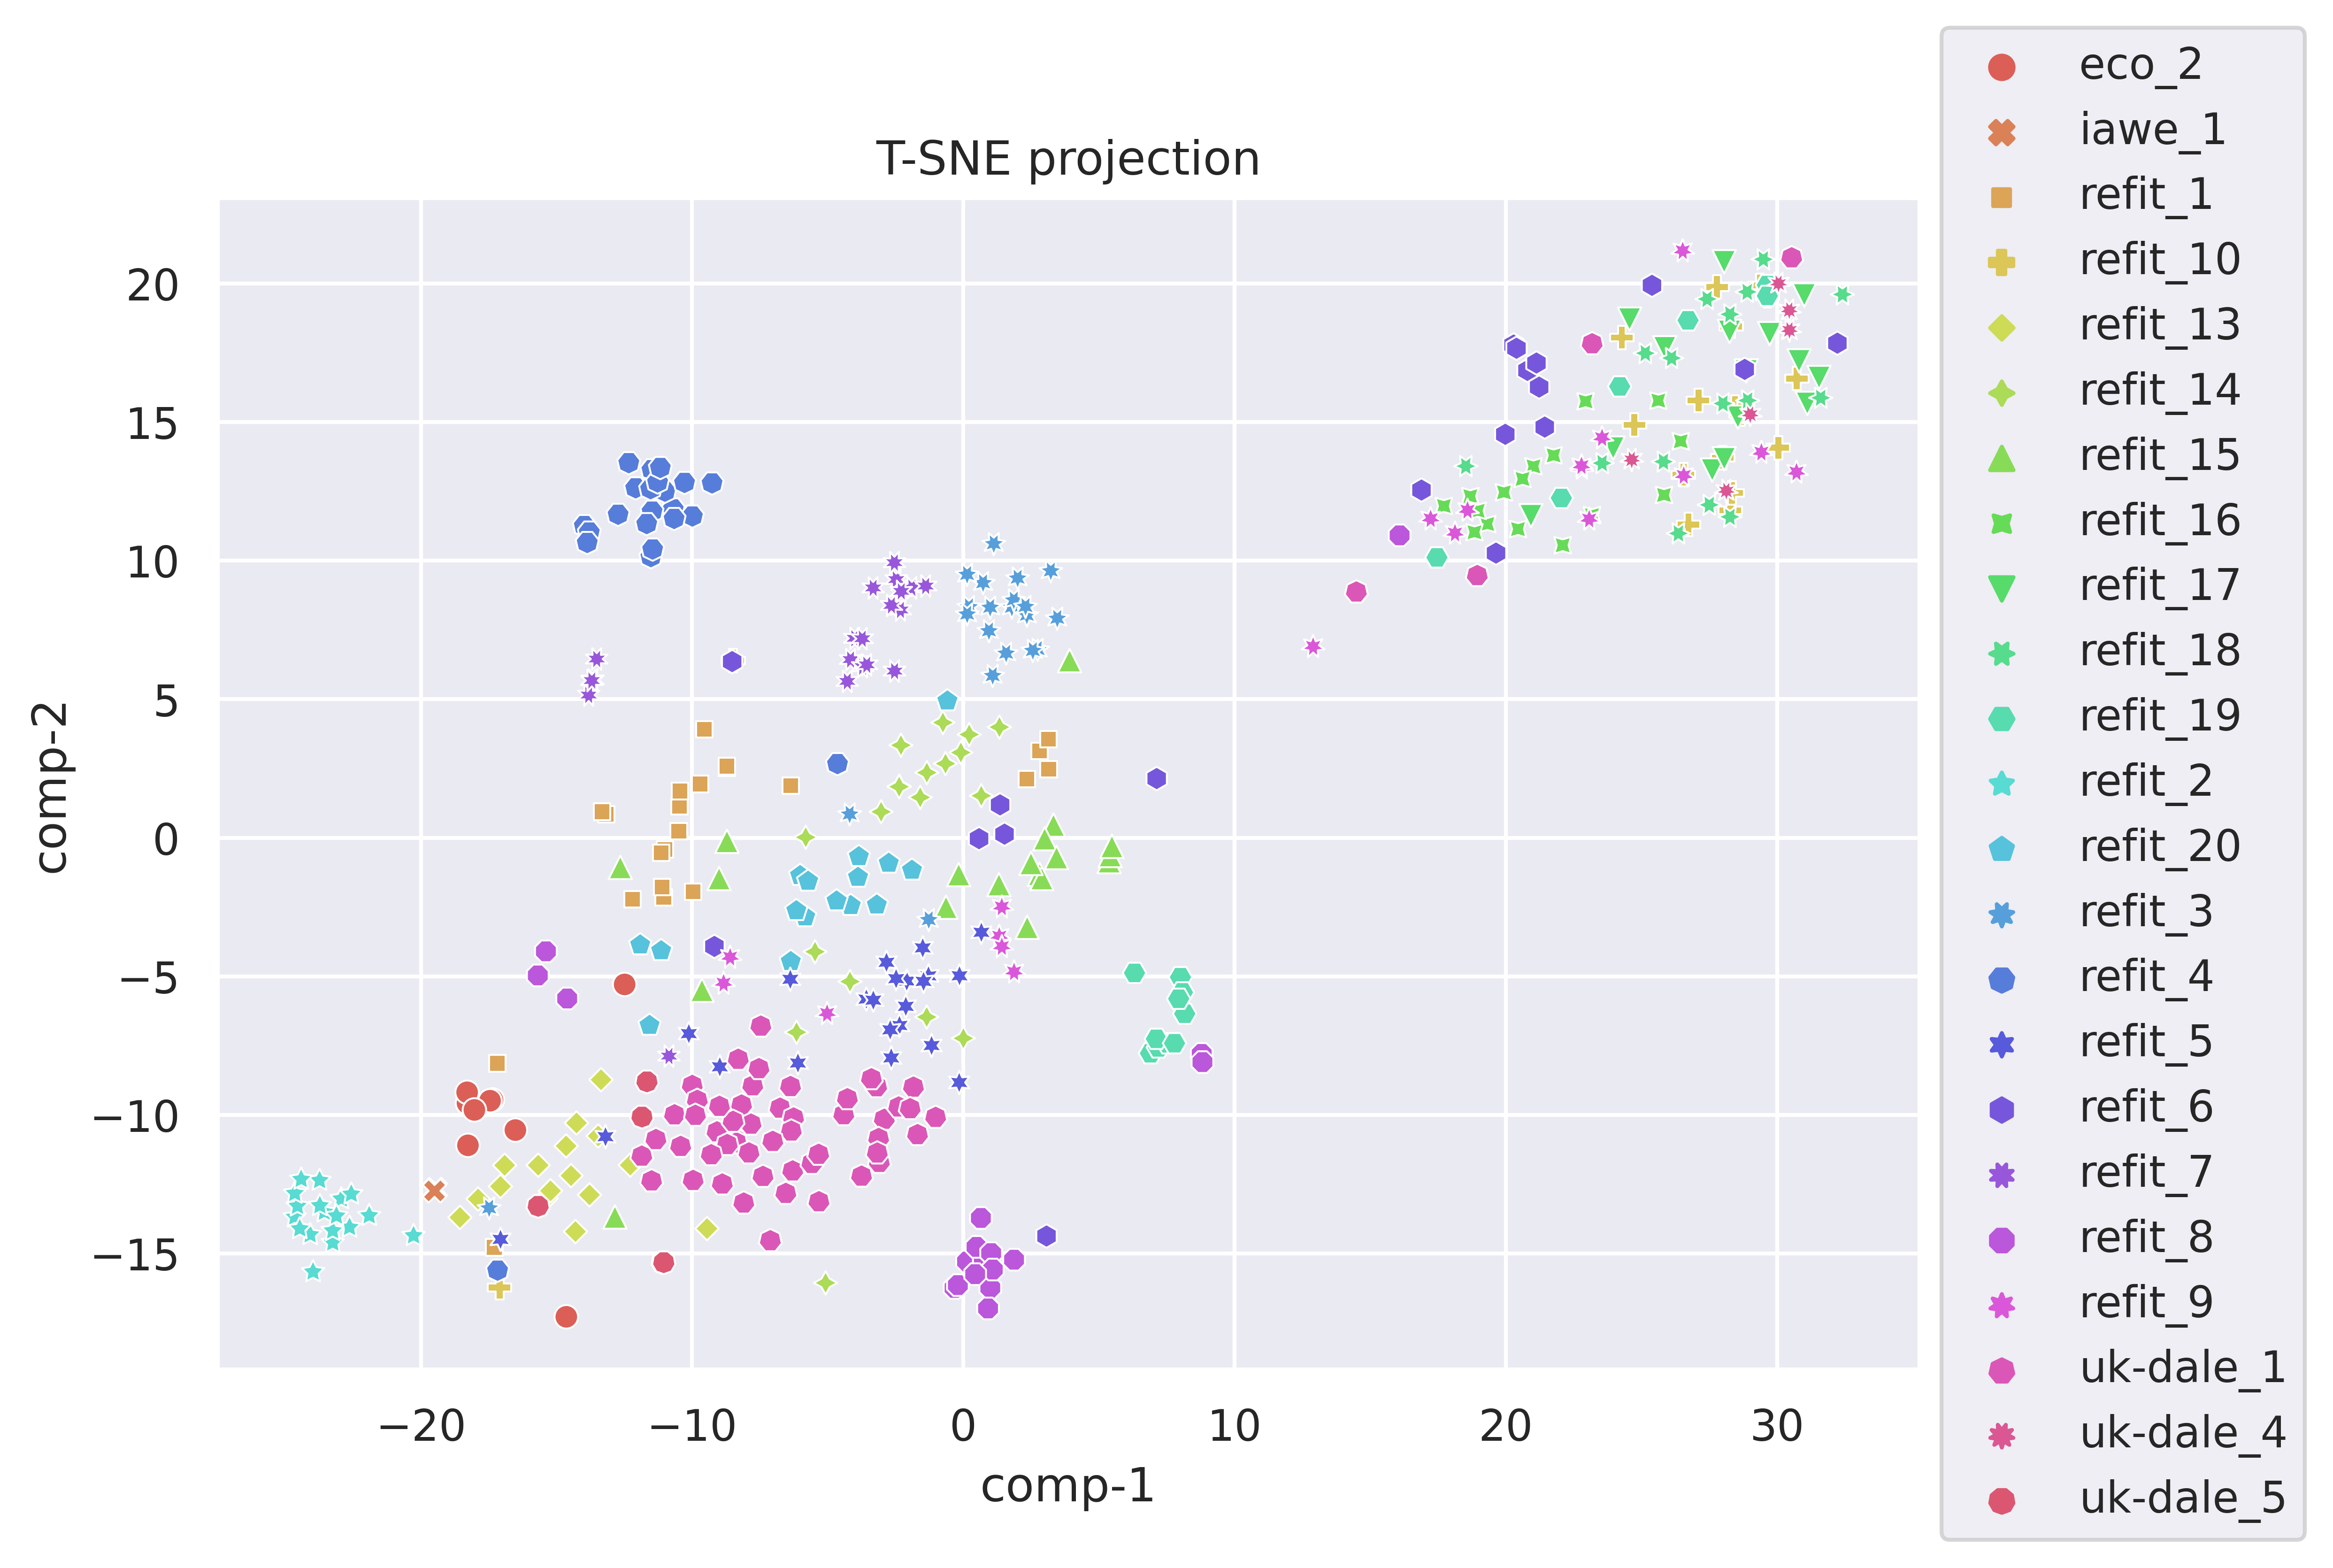
\includegraphics[width=1.2\textwidth]{Figures/TSNE/TSNE_per_appliance/all/scatter_all_television.png}
	\label{fig:tsne_pa_scatter_all_tv}
\end{figure}

The images on the figure behind clusters on proving the fact that outliers' consumption is a lot different.

\begin{figure}[H]
	\centering
	\caption{"Per appliance data for refit buildings images"}
	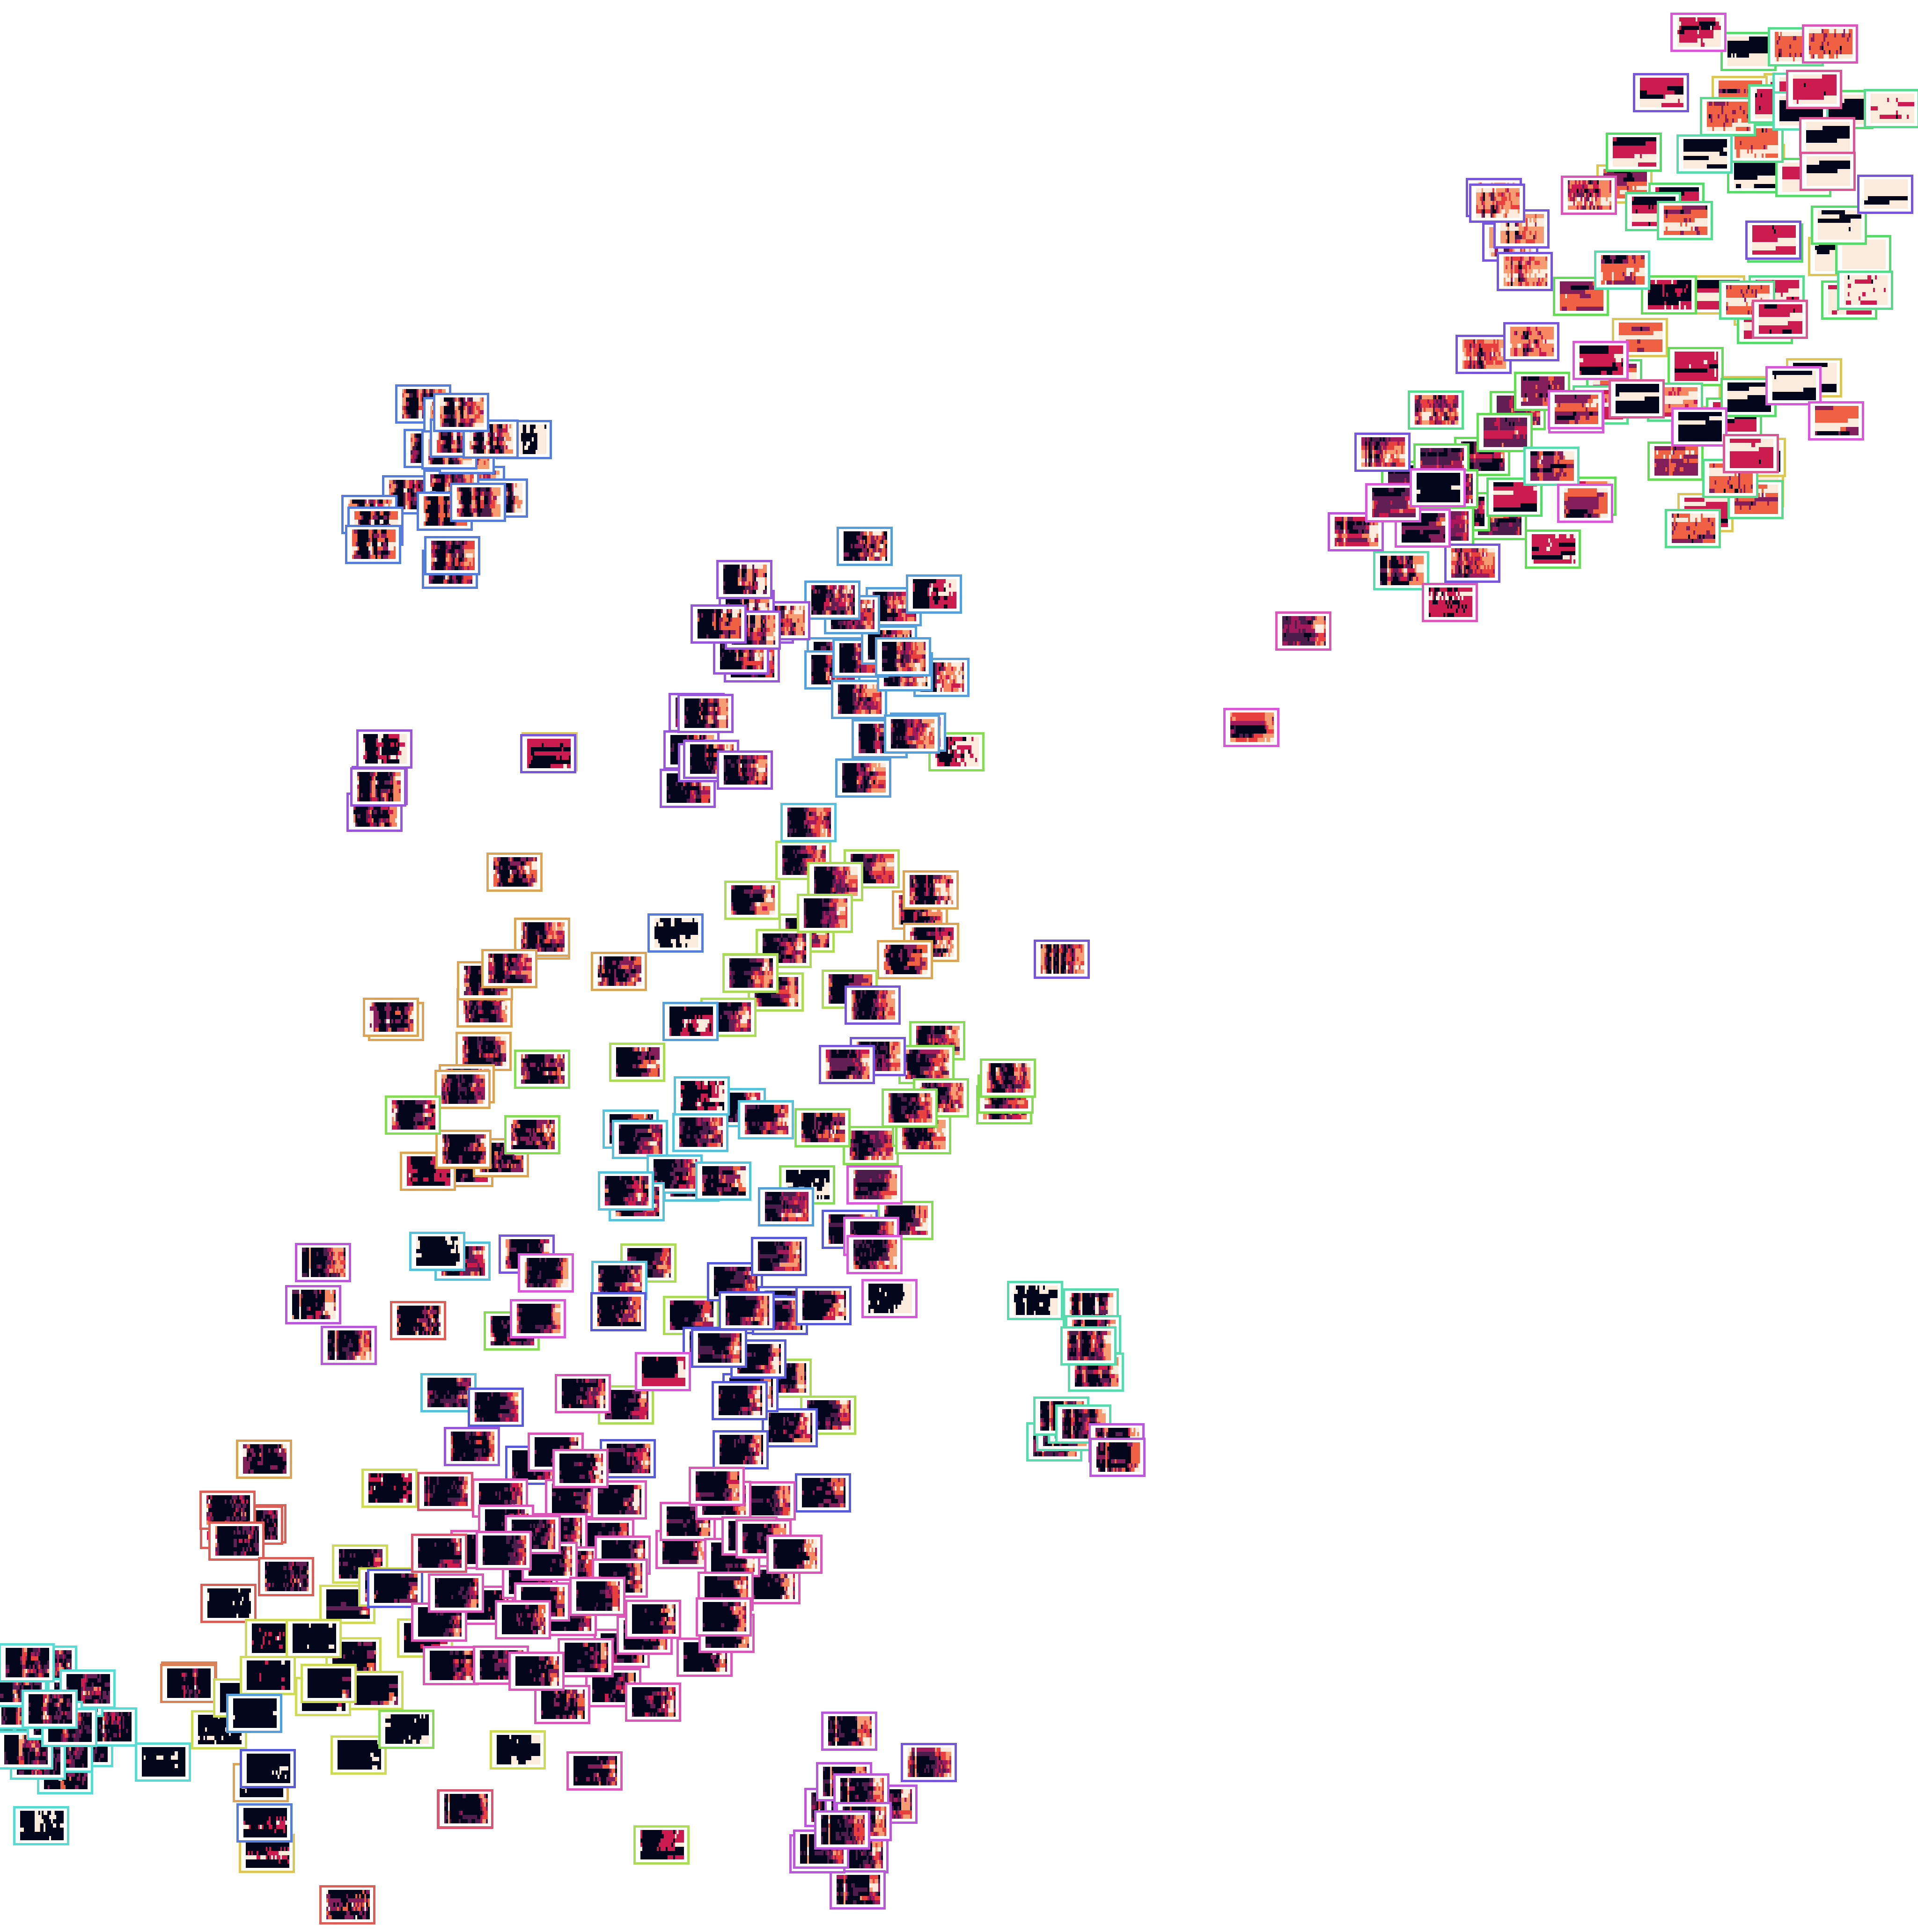
\includegraphics[width=.9\textwidth]{Figures/TSNE/TSNE_per_appliance/all/img_scatter_alltelevision.png}
	\label{fig:tsne_pa_img_scatter_all_tv}
\end{figure}

\subsubsection{Per appliance - comparing appliances}


The figure below \label{fig:tsne_papb_scatter_all} presents
the general picture where each appliance lays compared to other.

\begin{figure}[H]
	\centering
	\caption{"Per appliance per building data for all buildings"}
	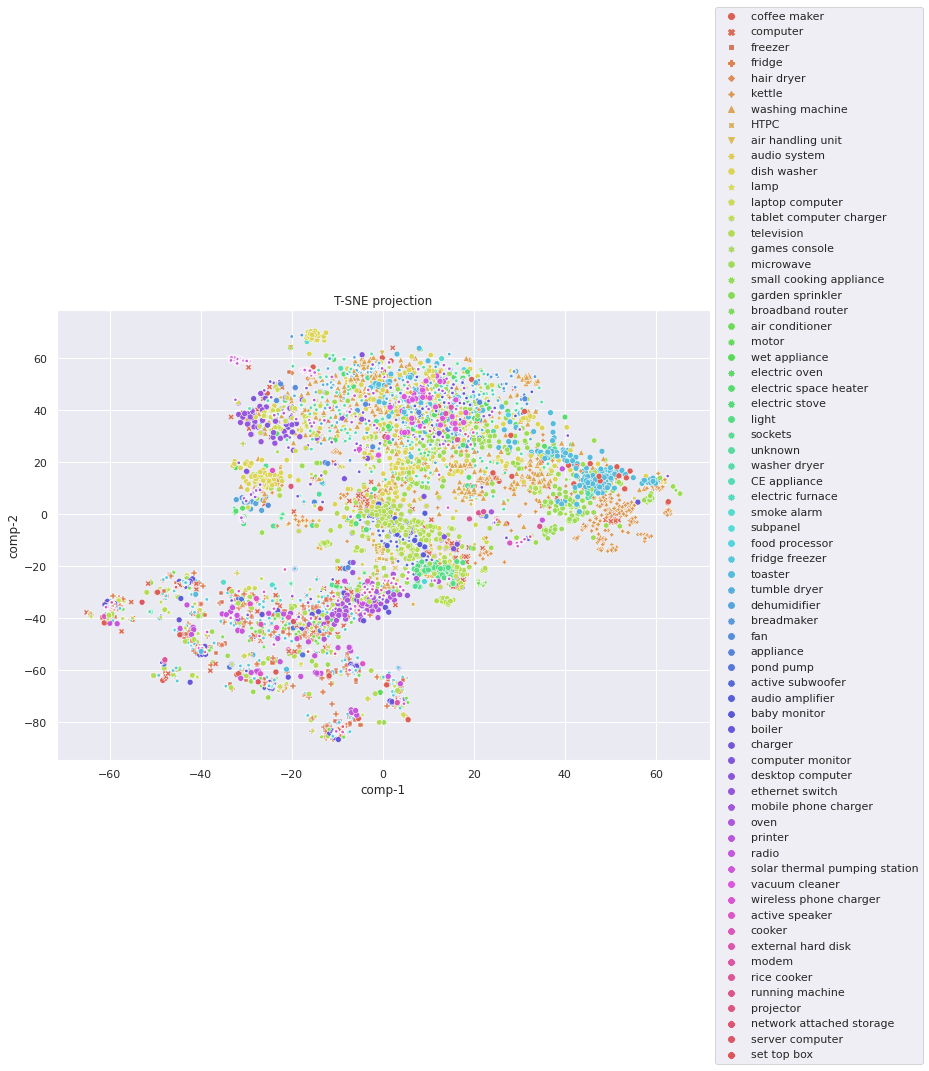
\includegraphics[width=1.2\textwidth]{Figures/TSNE/TSNE_results/all/scatter_all_all_lgimgs.png}
	\label{fig:tsne_papb_scatter_all}
\end{figure}

The same goes for imae presentation. We can clearly see, that
most active appliances are in the bottom left
and less activive appliances on the middle of upper cluster.

\begin{figure}[H]
	\centering
	\caption{"Per appliance data for refit buildings images"}
	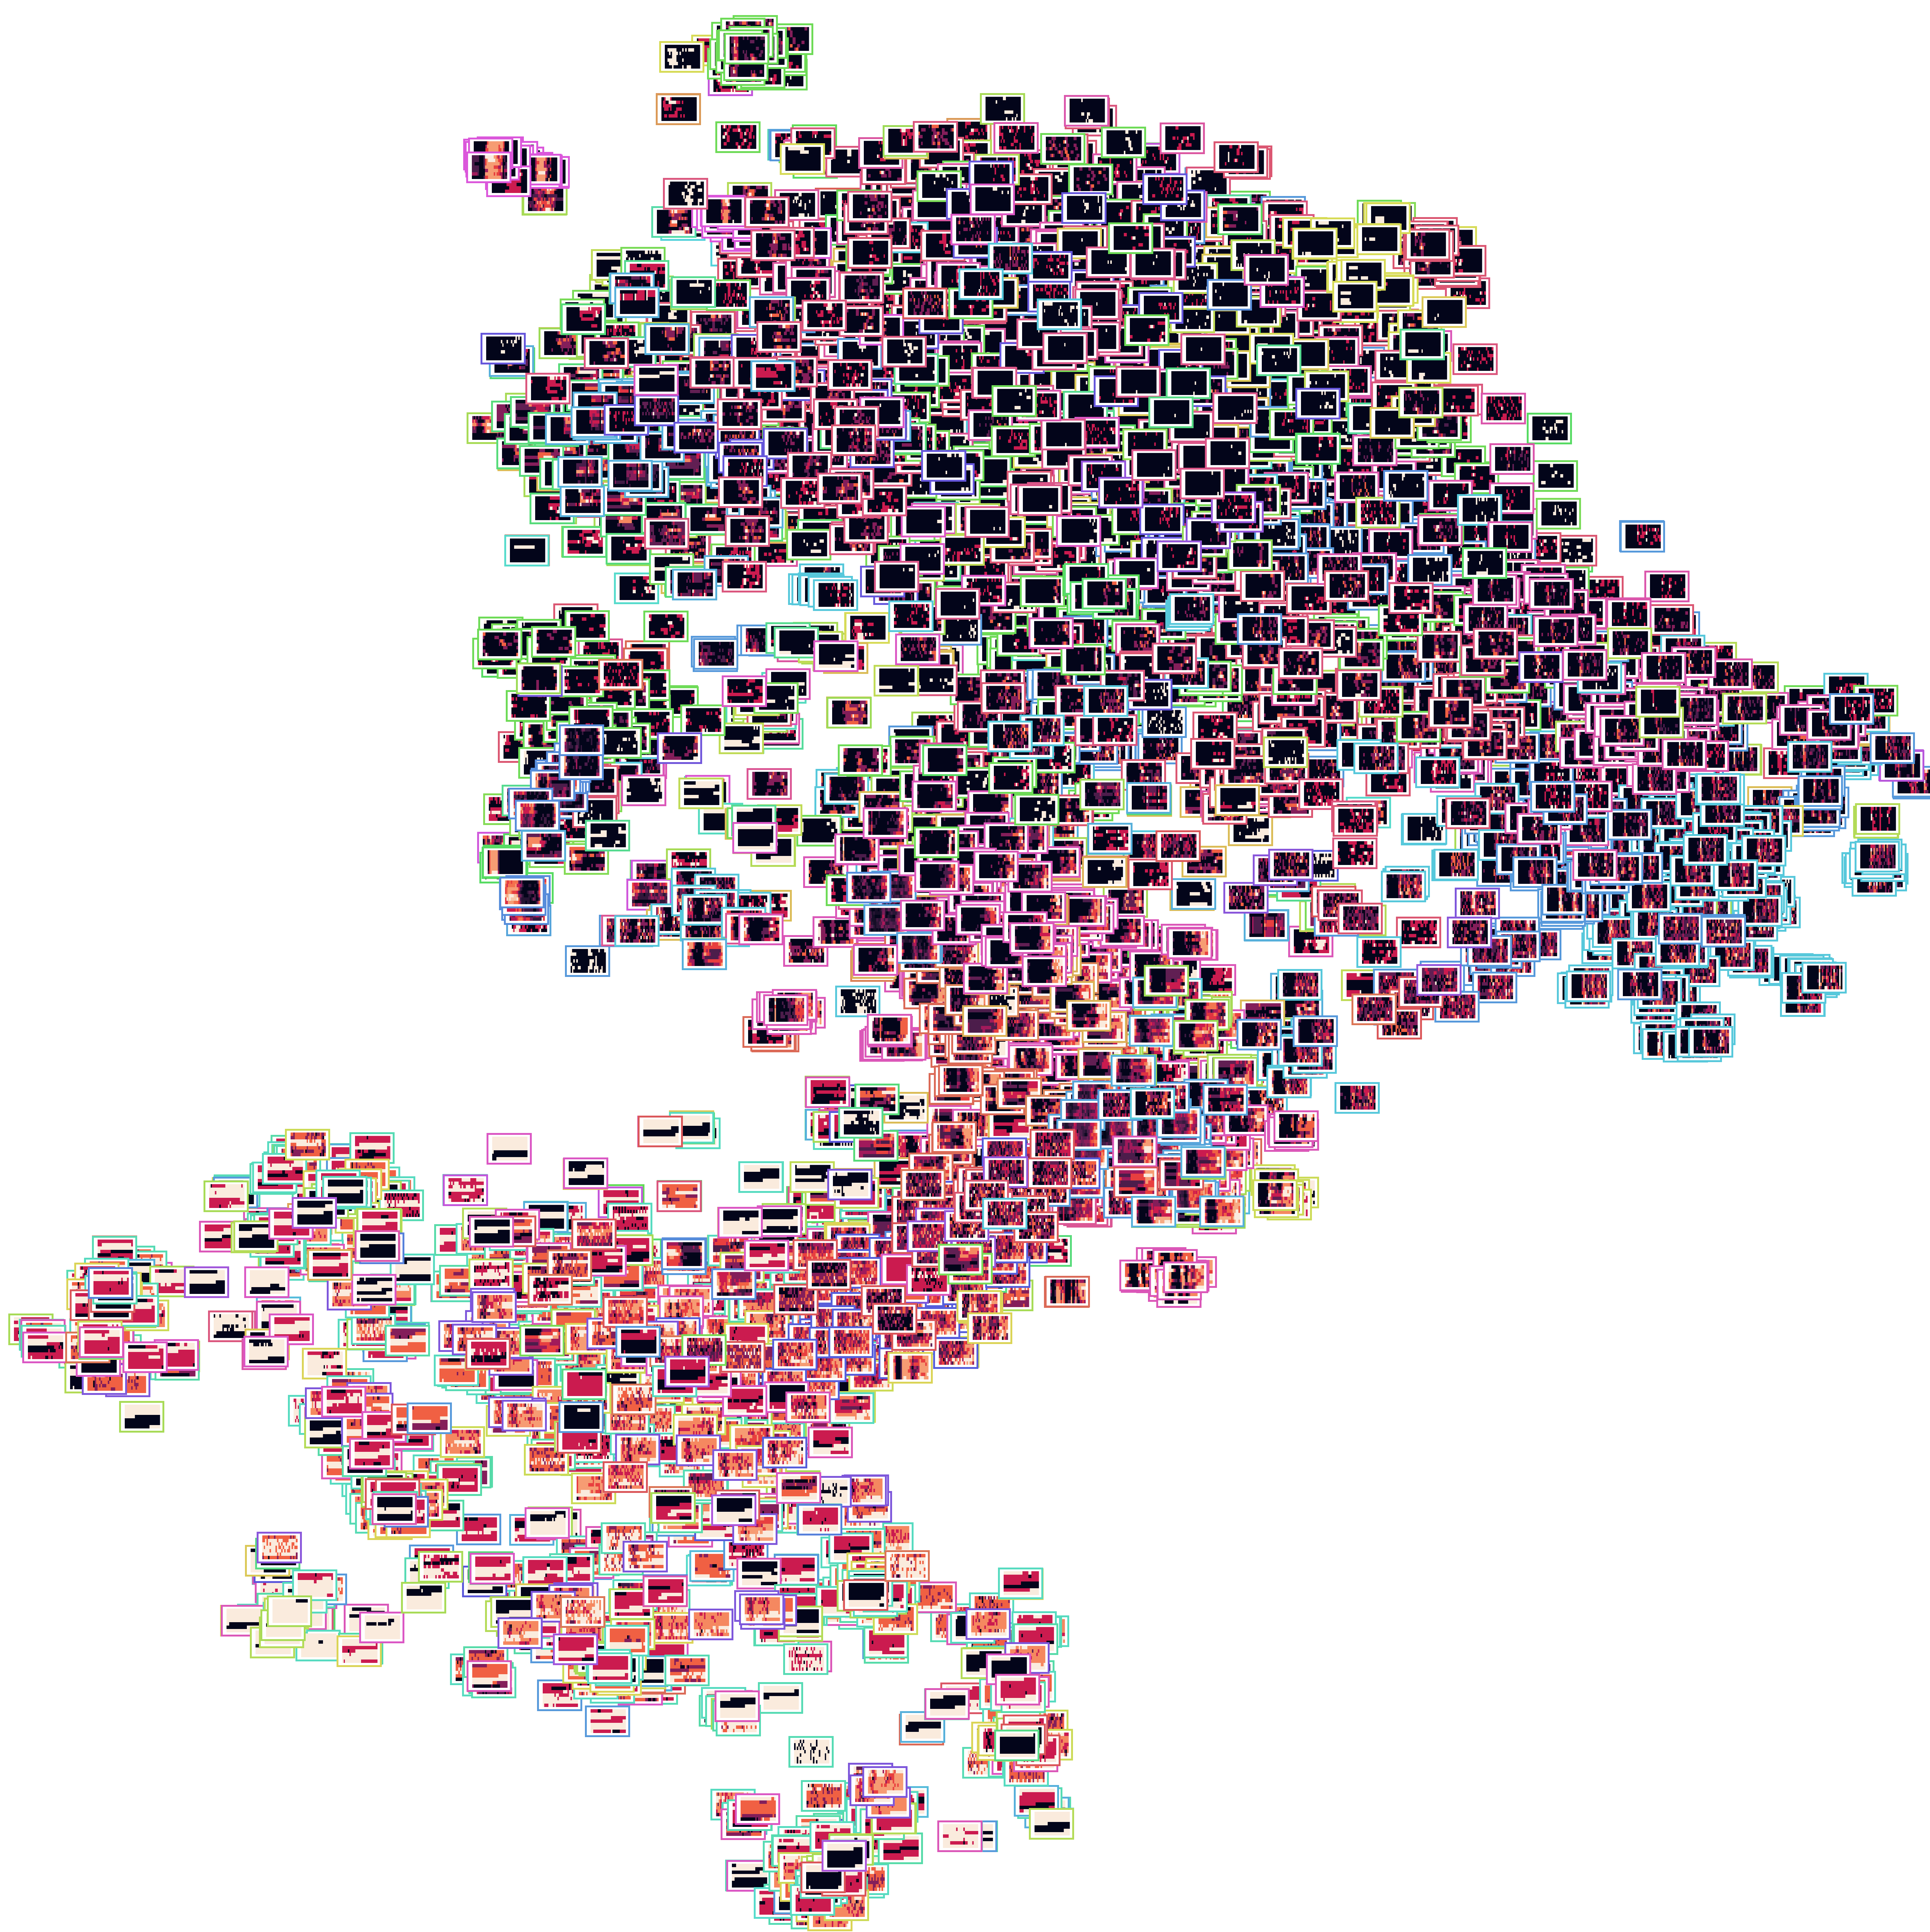
\includegraphics[width=.9\textwidth]{Figures/TSNE/TSNE_results/all/img_scatter_allall_lgimgs.png}
	\label{fig:tsne_papb_img_scatter_all}
\end{figure}

The issue here is, that there are to many appliances, and this
causes the legend to be to populated.


In order to get general idea where each appliance group lies,
lets filter out all appliances that have less that 150 samples.
Appliing this filter yileds figure \ref{fig:tsne_papb_scatter_all_reduced}.

\begin{figure}[H]
	\centering
	\caption{"Per appliance per building data for all buildings"}
	\includegraphics[width=1.1\textwidth]{Figures/TSNE/TSNE_results/all/scatter_all_all_reduced_max.png}
	\label{fig:tsne_papb_scatter_all_reduced}
\end{figure}

It is posible to se how these 10 appliances ares connected in high dimensional space.
It is possible that similar appliances are near eachoter.
Kettle, microwave and toaster are quite similar.
They have short operaring times, and are usually used in users routine.
These appliances are located in the upper left part of the plot.
Second group of appliances that are quite near eachother are white
goods (without fridges) such as washing machine, dishashers etc.
Lets say that they are with goods with a program. 
This group of appliances says in the upper right part of the plot.
The other group of appliances are withe goods with a compressor.
They are usualy not affecet by human interaction, and are 
therefore hard to cluster. They take a part in the whole lower part of the plot.
Final group of appliances are TVs and computers. They lie 
on a bridge between the fridges and other groups. 

\begin{figure}[H]
	\centering
	\caption{"Per appliance data for refit buildings images"}
	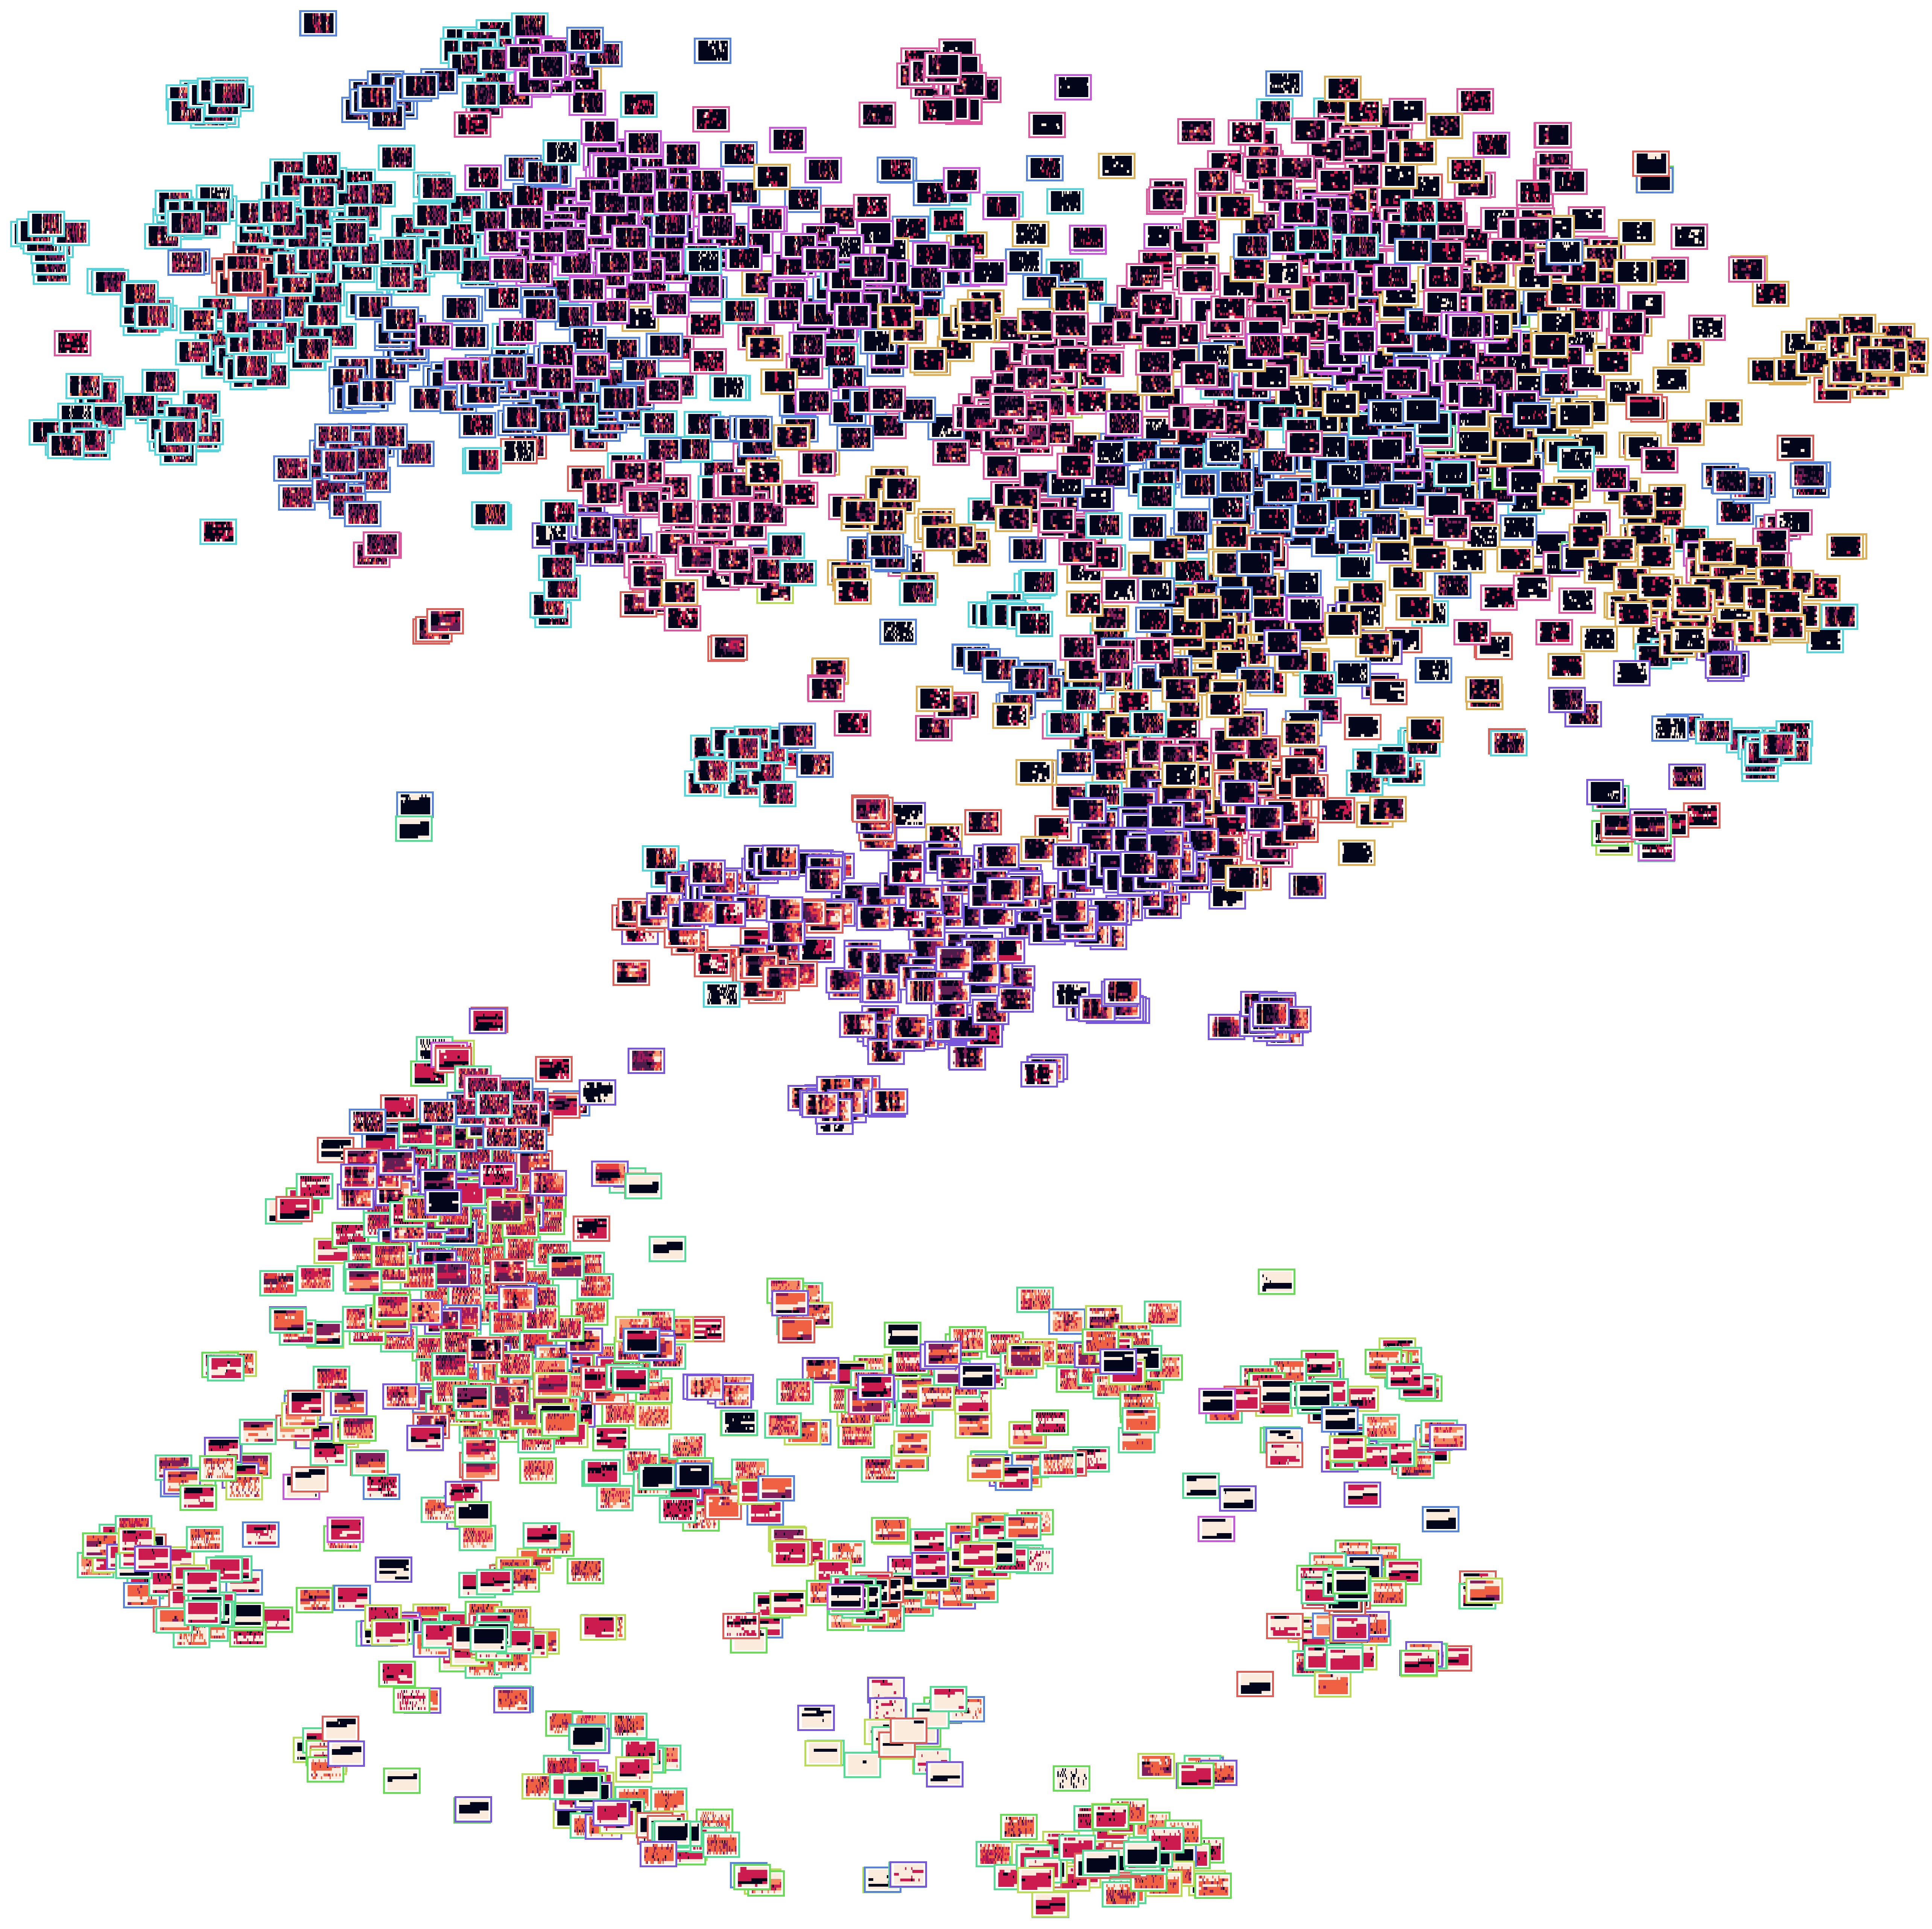
\includegraphics[width=.9\textwidth]{Figures/TSNE/TSNE_results/all/img_scatter_allall_reduced_max.png}
	\label{fig:tsne_papb_img_scatter_all_reduced}
\end{figure}

All trough the dataset is different due to filtering,
the figure \ref{fig:tsne_papb_img_scatter_all_reduced},
retains similar structure to the previous picture. 

\subsection{group appliances}

Knowing that a pattern exist, and using the rough pattern 
we can define appliance groups. 
8 appliance groups will be defined.

\begin{itemize}
    \item Kitchen appliances - toasters, ovens, microwaves etc
    \item Fridges and freeezer  - contains fridges frezers and fridge freezers
    \item White goods - washers, dryers, dish washers i.e white goods with a program
    \item heating and cooling - Electric radiators, dehumudifiers and HVACS
    \item leisure - Usualy living room appliances such as TVs, games consles, audio amps, HTPCs
    \item home office - Computer, laptops, printers, network equipment, chargers
    \item lightning - lights and lamps
    \item Others - unknown applainces, unlabeled
\end{itemize}

Appliing these groups yileds figure \ref{fig:tsne_papb_scatter_all_groups}.
The new plot shows how that altrough appliances could be used by a different
user, maybe even by user in a diffent part of the EU or world,
they can be grouped in a high dimensonal space. 
\begin{figure}[H]
	\centering
	\caption{"Per appliance per building data for all buildings"}
	\includegraphics[width=.8\textwidth]{Figures/TSNE/TSNE_results/all/scatter_all_all_groups.png}
	\label{fig:tsne_papb_scatter_all_groups}
\end{figure}

The image beloow is the same as the first one in the subsection,
exept it is easier to use color to see the appliance they present

\begin{figure}[H]
	\centering
	\caption{"Per appliance data for refit buildings images"}
	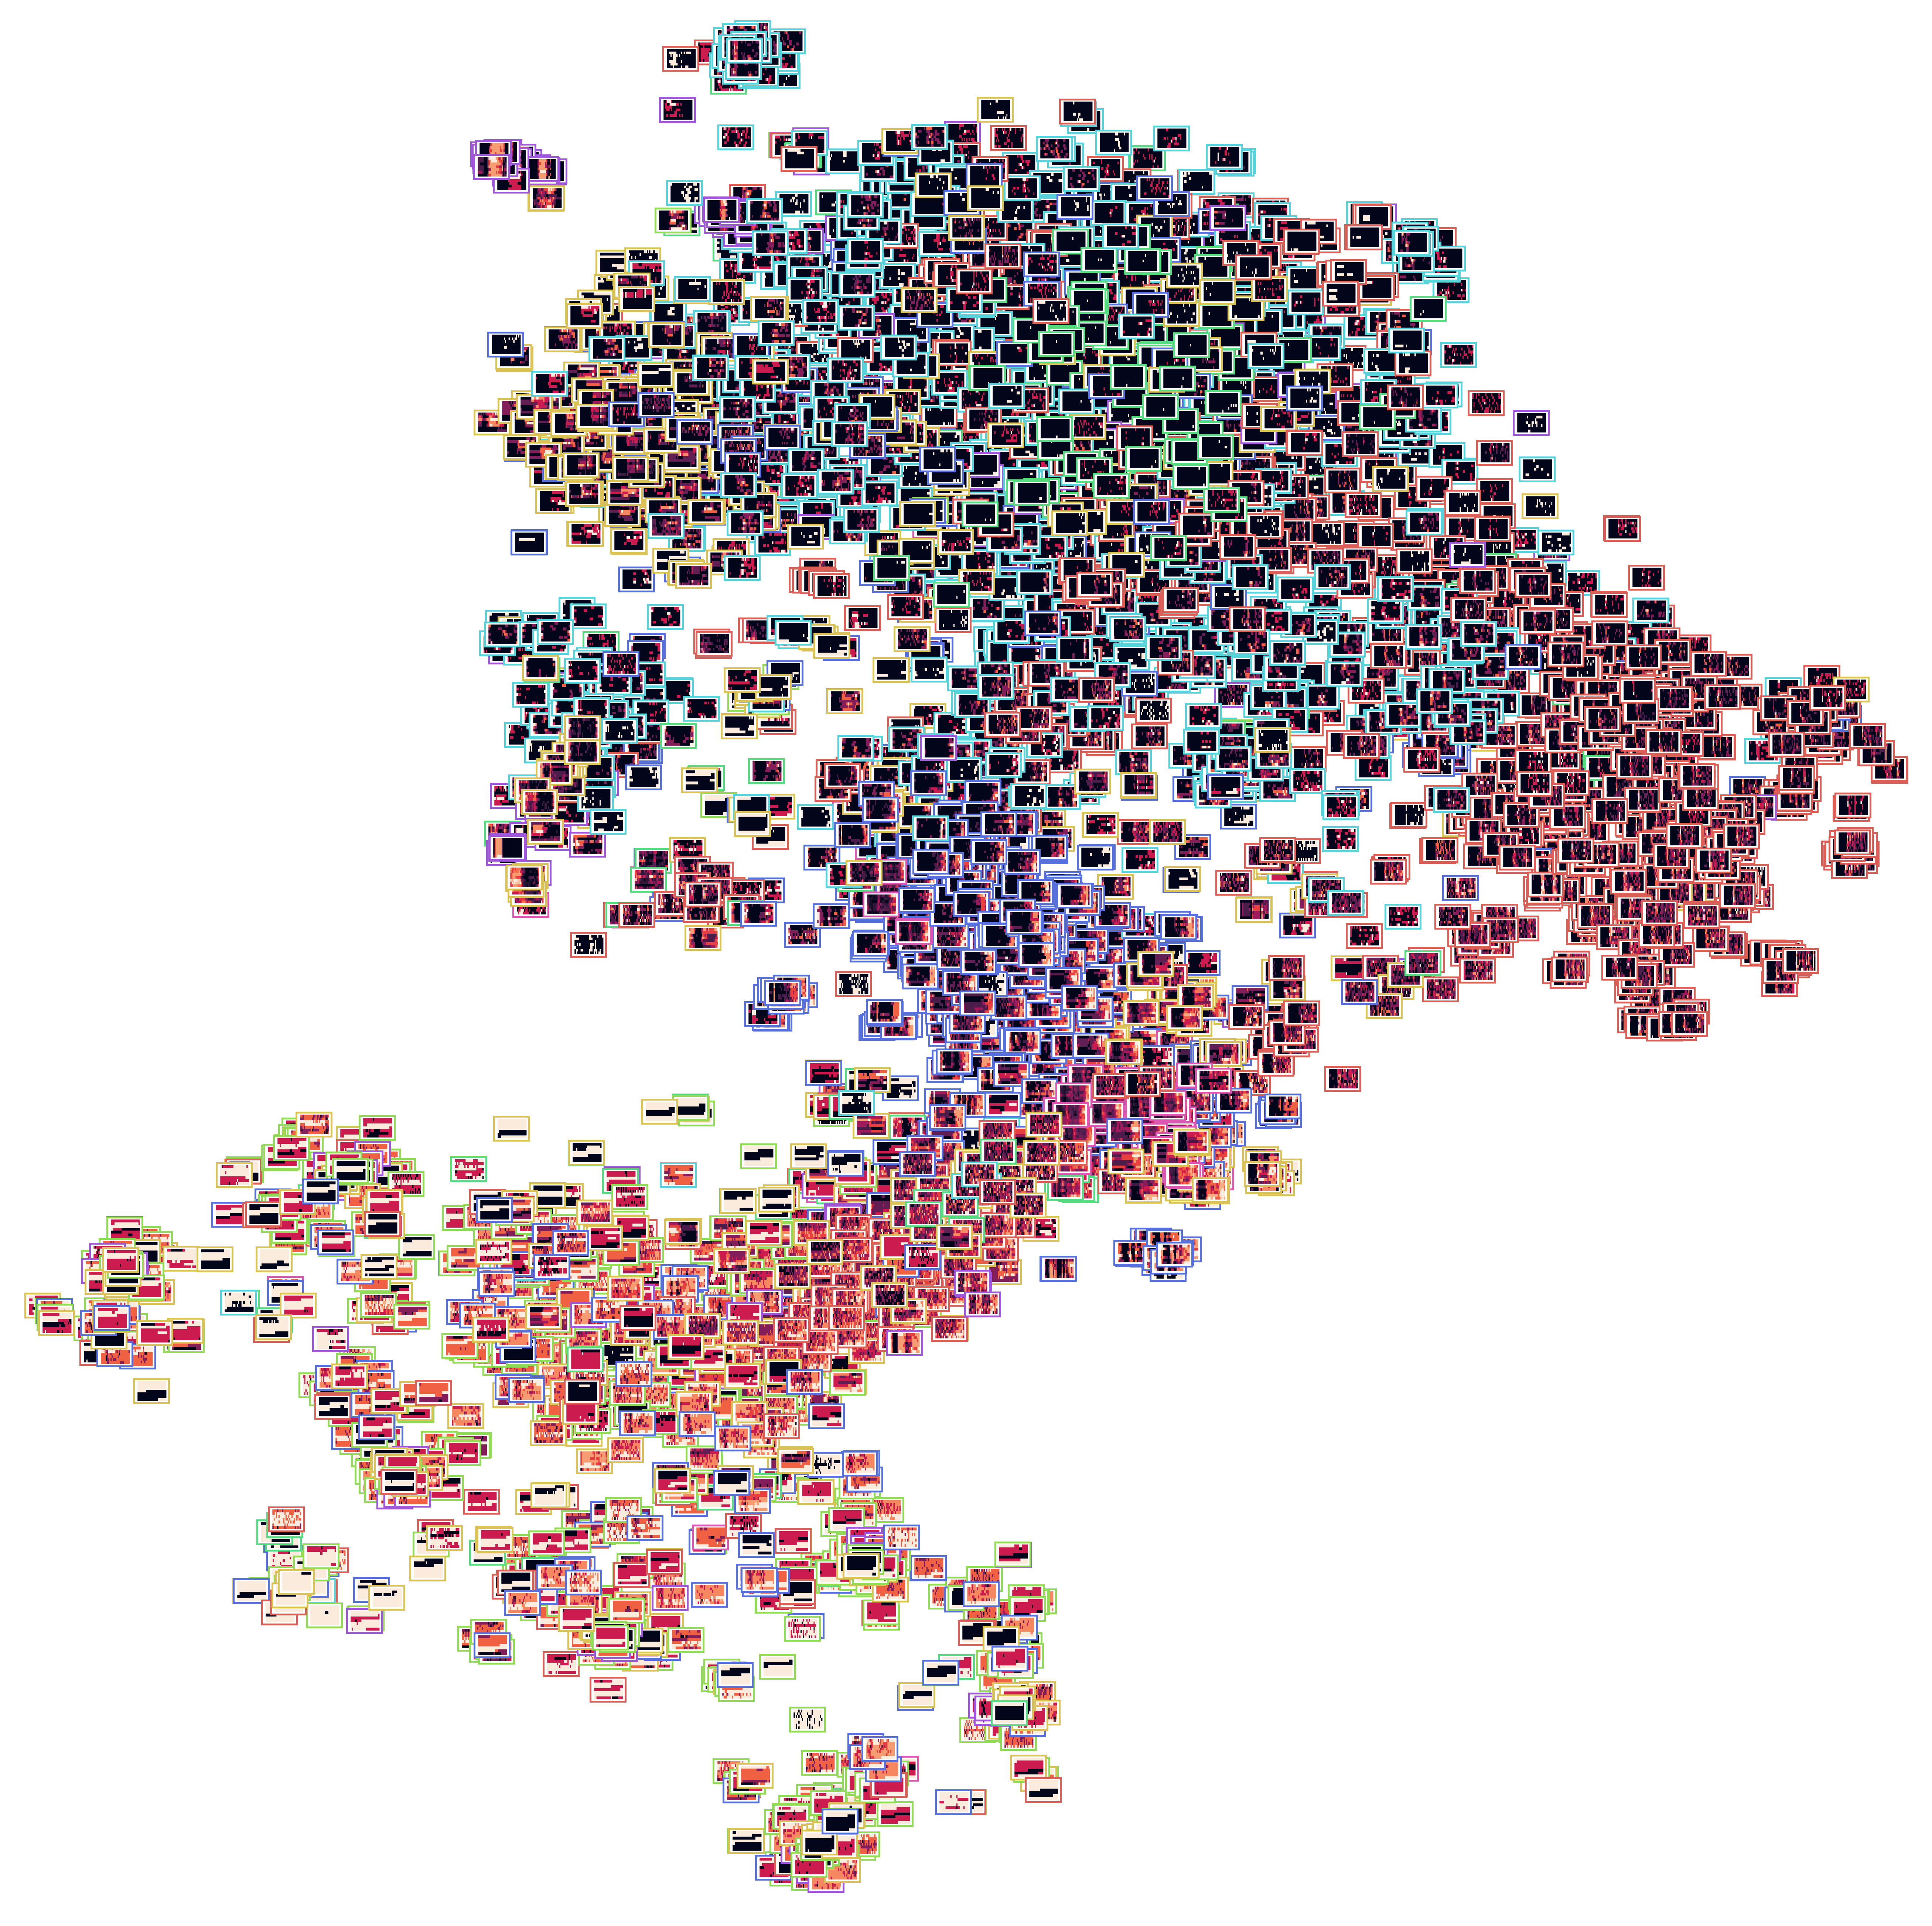
\includegraphics[width=.9\textwidth]{Figures/TSNE/TSNE_results/all/img_scatter_all_all_groups.png}
	\label{fig:tsne_papb_img_scatter_all_groups}
\end{figure}

\subsection{filter low entropy}

One issue that causes the t-SNE algorim an issue is low entropy data or 
in other words images that are almost completly dark or white.

If we calculate entropy for each image and set some low treshold
it is possible to filter out these samples. 
Setting an entropy trehold of 0.5, we filter out around 5 \%
of all samples. 

\begin{figure}[H]
	\centering
	\caption{"Per appliance per building data for all buildings"}
	\includegraphics[width=.8\textwidth]{Figures/TSNE/TSNE_results_entropy/all/scatter_all_all.png}
	\label{fig:tsne_papb_scatter_ent_all_groups}
\end{figure}

Again, we can apply groups and get a bit more a bit nicer clusters. 

\begin{figure}[H]
	\centering
	\caption{"Per appliance per building data for all buildings"}
	\includegraphics[width=.8\textwidth]{Figures/TSNE/TSNE_results_entropy/all/scatter_all_all_groups.png}
	\label{fig:tsne_papb_img_scatter_ent_all_groups}
\end{figure}


\subsubsection{single buildings}

It is also possible to use per appliance data to study
individual buidlings, and how each appliance is used here

\begin{figure}[H]
	\centering
	\caption{"Per appliance per building data for all buildings"}
	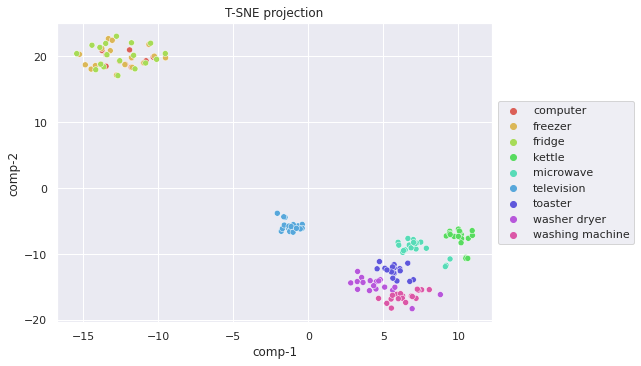
\includegraphics[width=.8\textwidth]{Figures/TSNE/TSNE_results/refit/scatter_refit_8.png}
	\label{fig:tsne_papb_scatter_ent_refit8}
\end{figure}

In general, the stricture is similar to before.
fridge and freezers are outliers and TV in somewhere in between.

\begin{figure}[H]
	\centering
	\caption{"Per appliance data for refit buildings images"}
	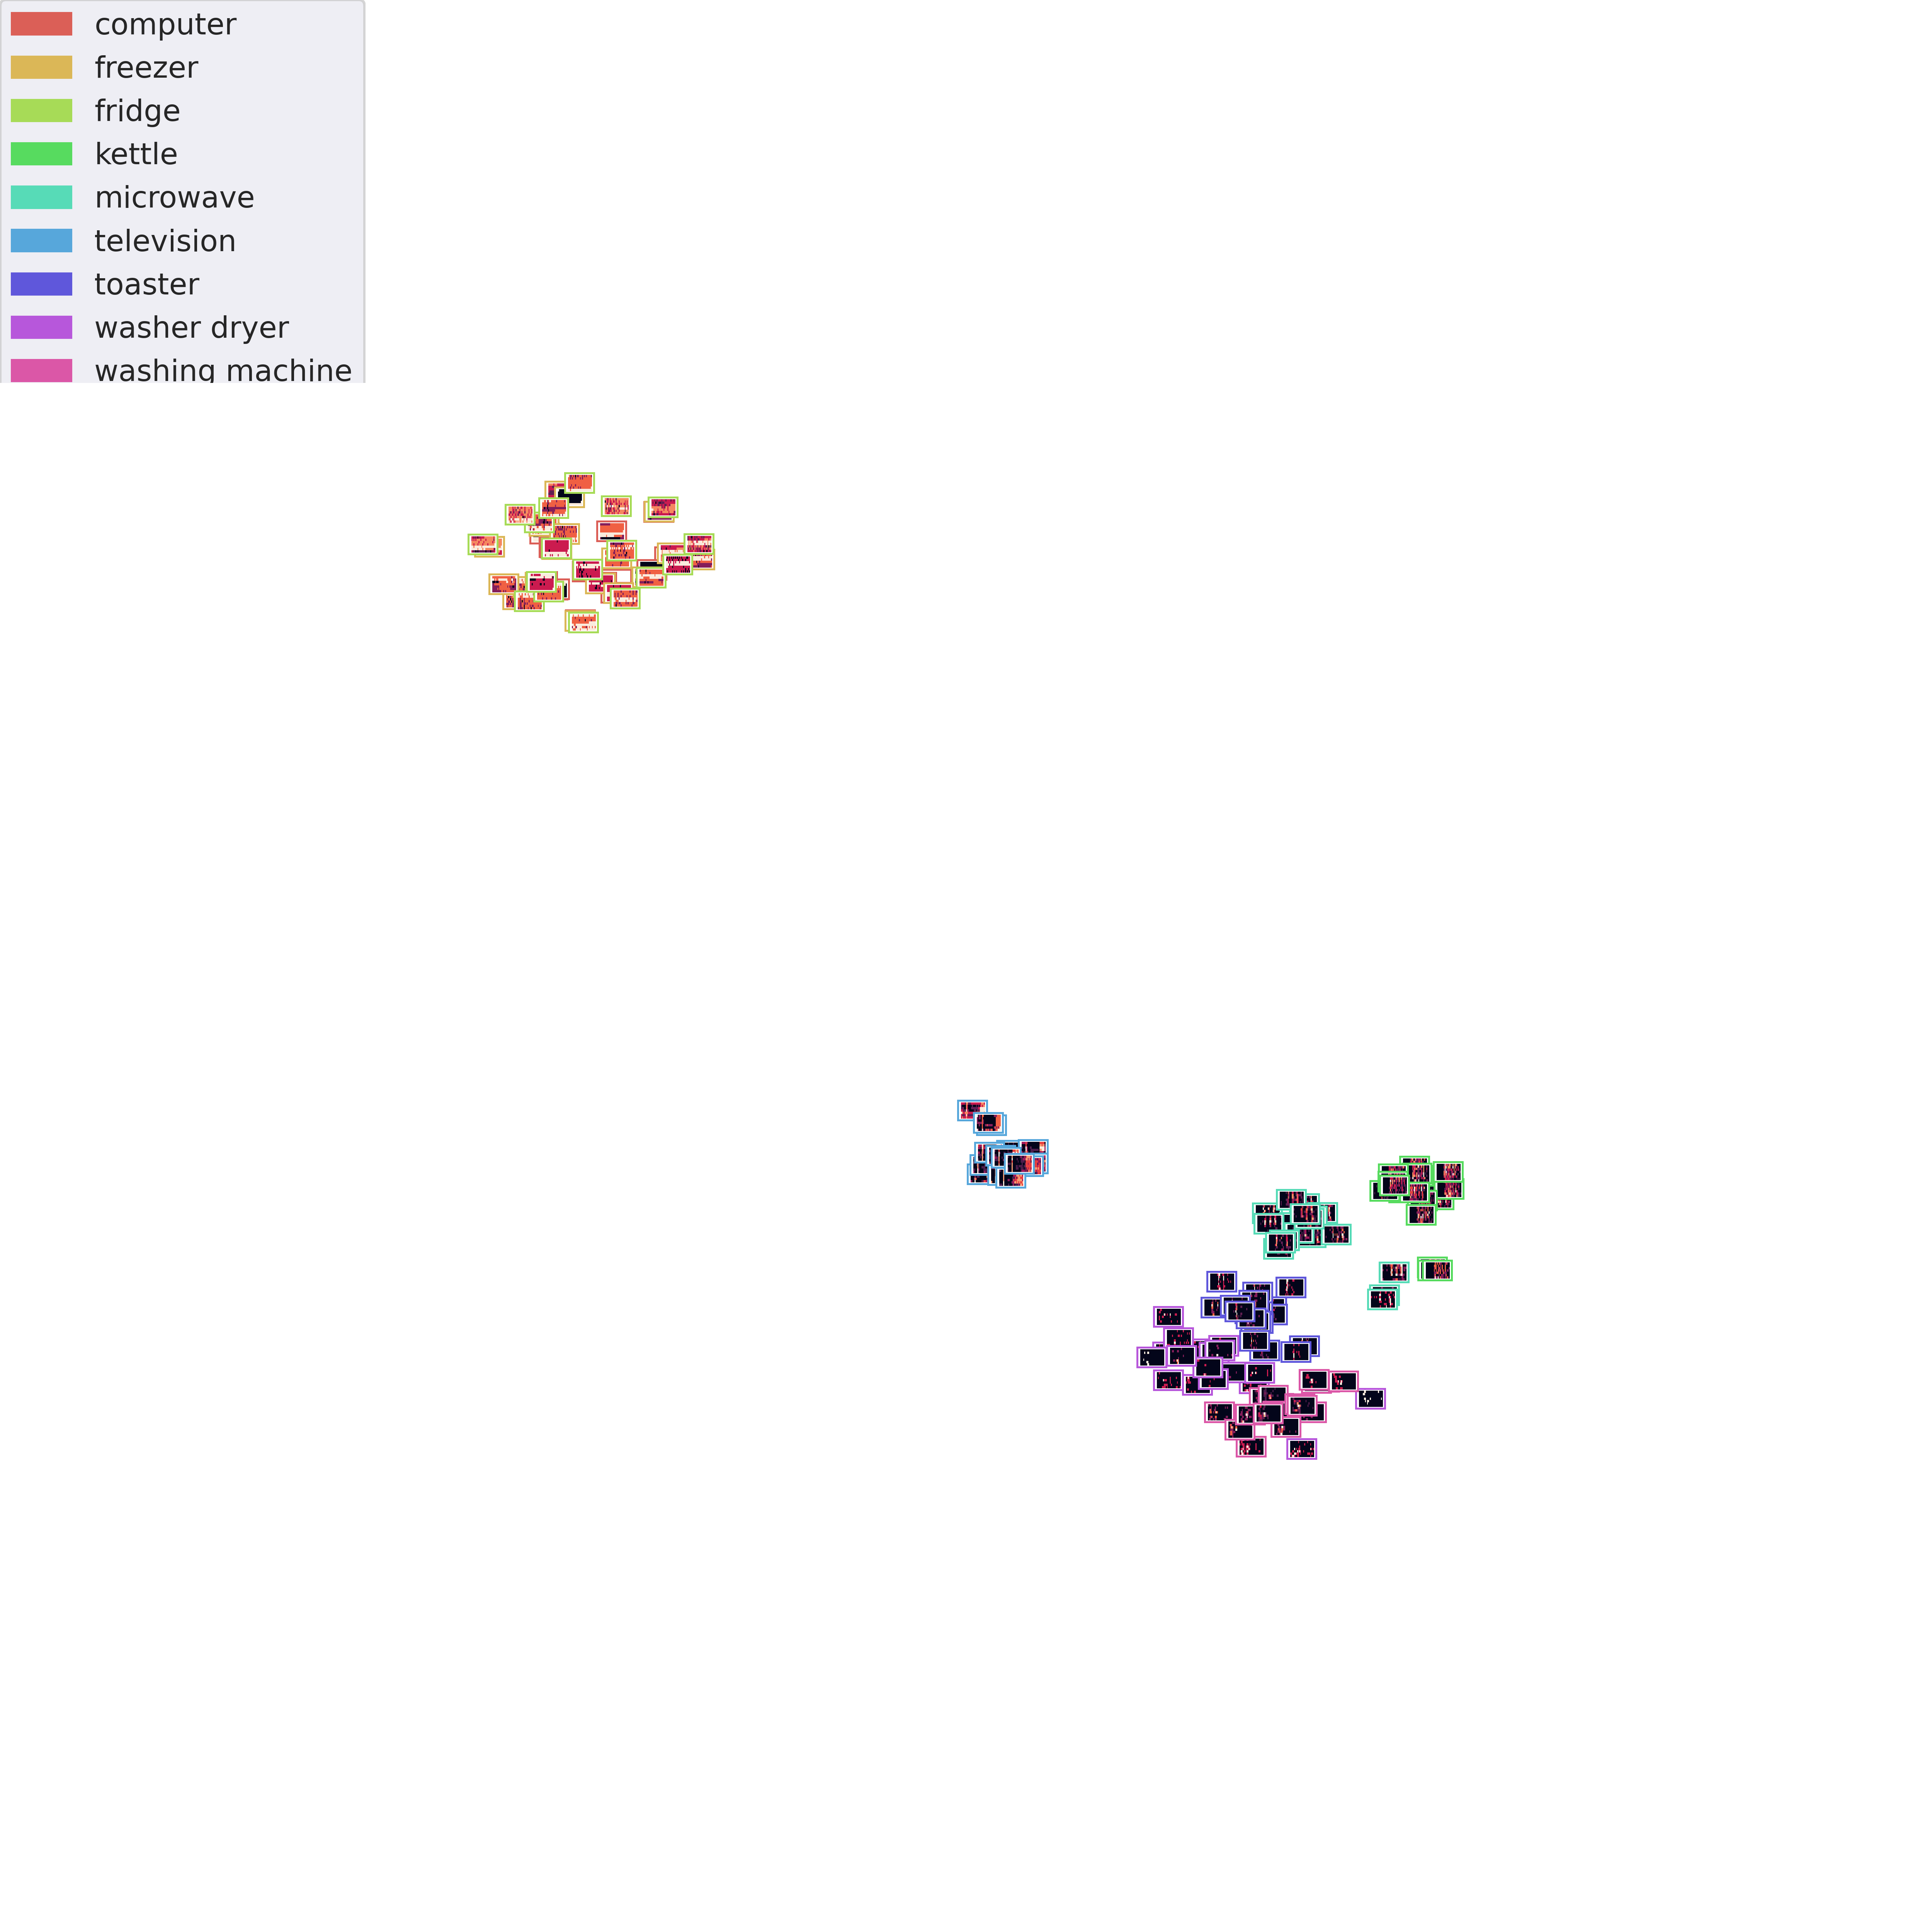
\includegraphics[width=.9\textwidth]{Figures/TSNE/TSNE_results/refit/img_scatter_refit8.png}
	\label{fig:tsne_papb_img_scatter_ent_refit8}
\end{figure}


\subsection{Per-appliance per-building}
To study the usage comparing all appliances between buildings,
we have to use a proposed type of profile.

\subsubsection{Bag off appliances}
This profile is called bag of appliances, and 
enables us to compare usage between buildings

\begin{figure}[H]
	\centering
	\caption{"Per appliance per building data for all buildings"}
	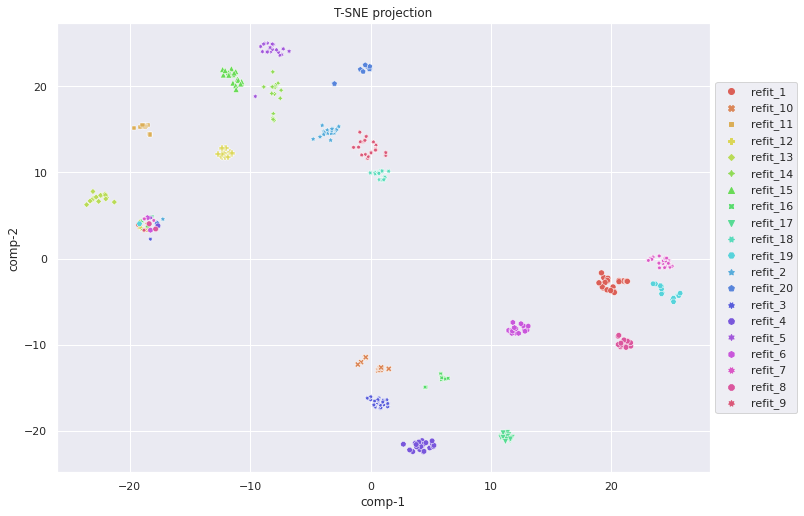
\includegraphics[width=.8\textwidth]{Figures/TSNE/TSNE_BOA/refit/scatter_refit_all.png}
	\label{fig:tsne_boa_scatter_refit8}
\end{figure}


\begin{figure}[H]
	\centering
	\caption{"Per appliance data for refit buildings images"}
	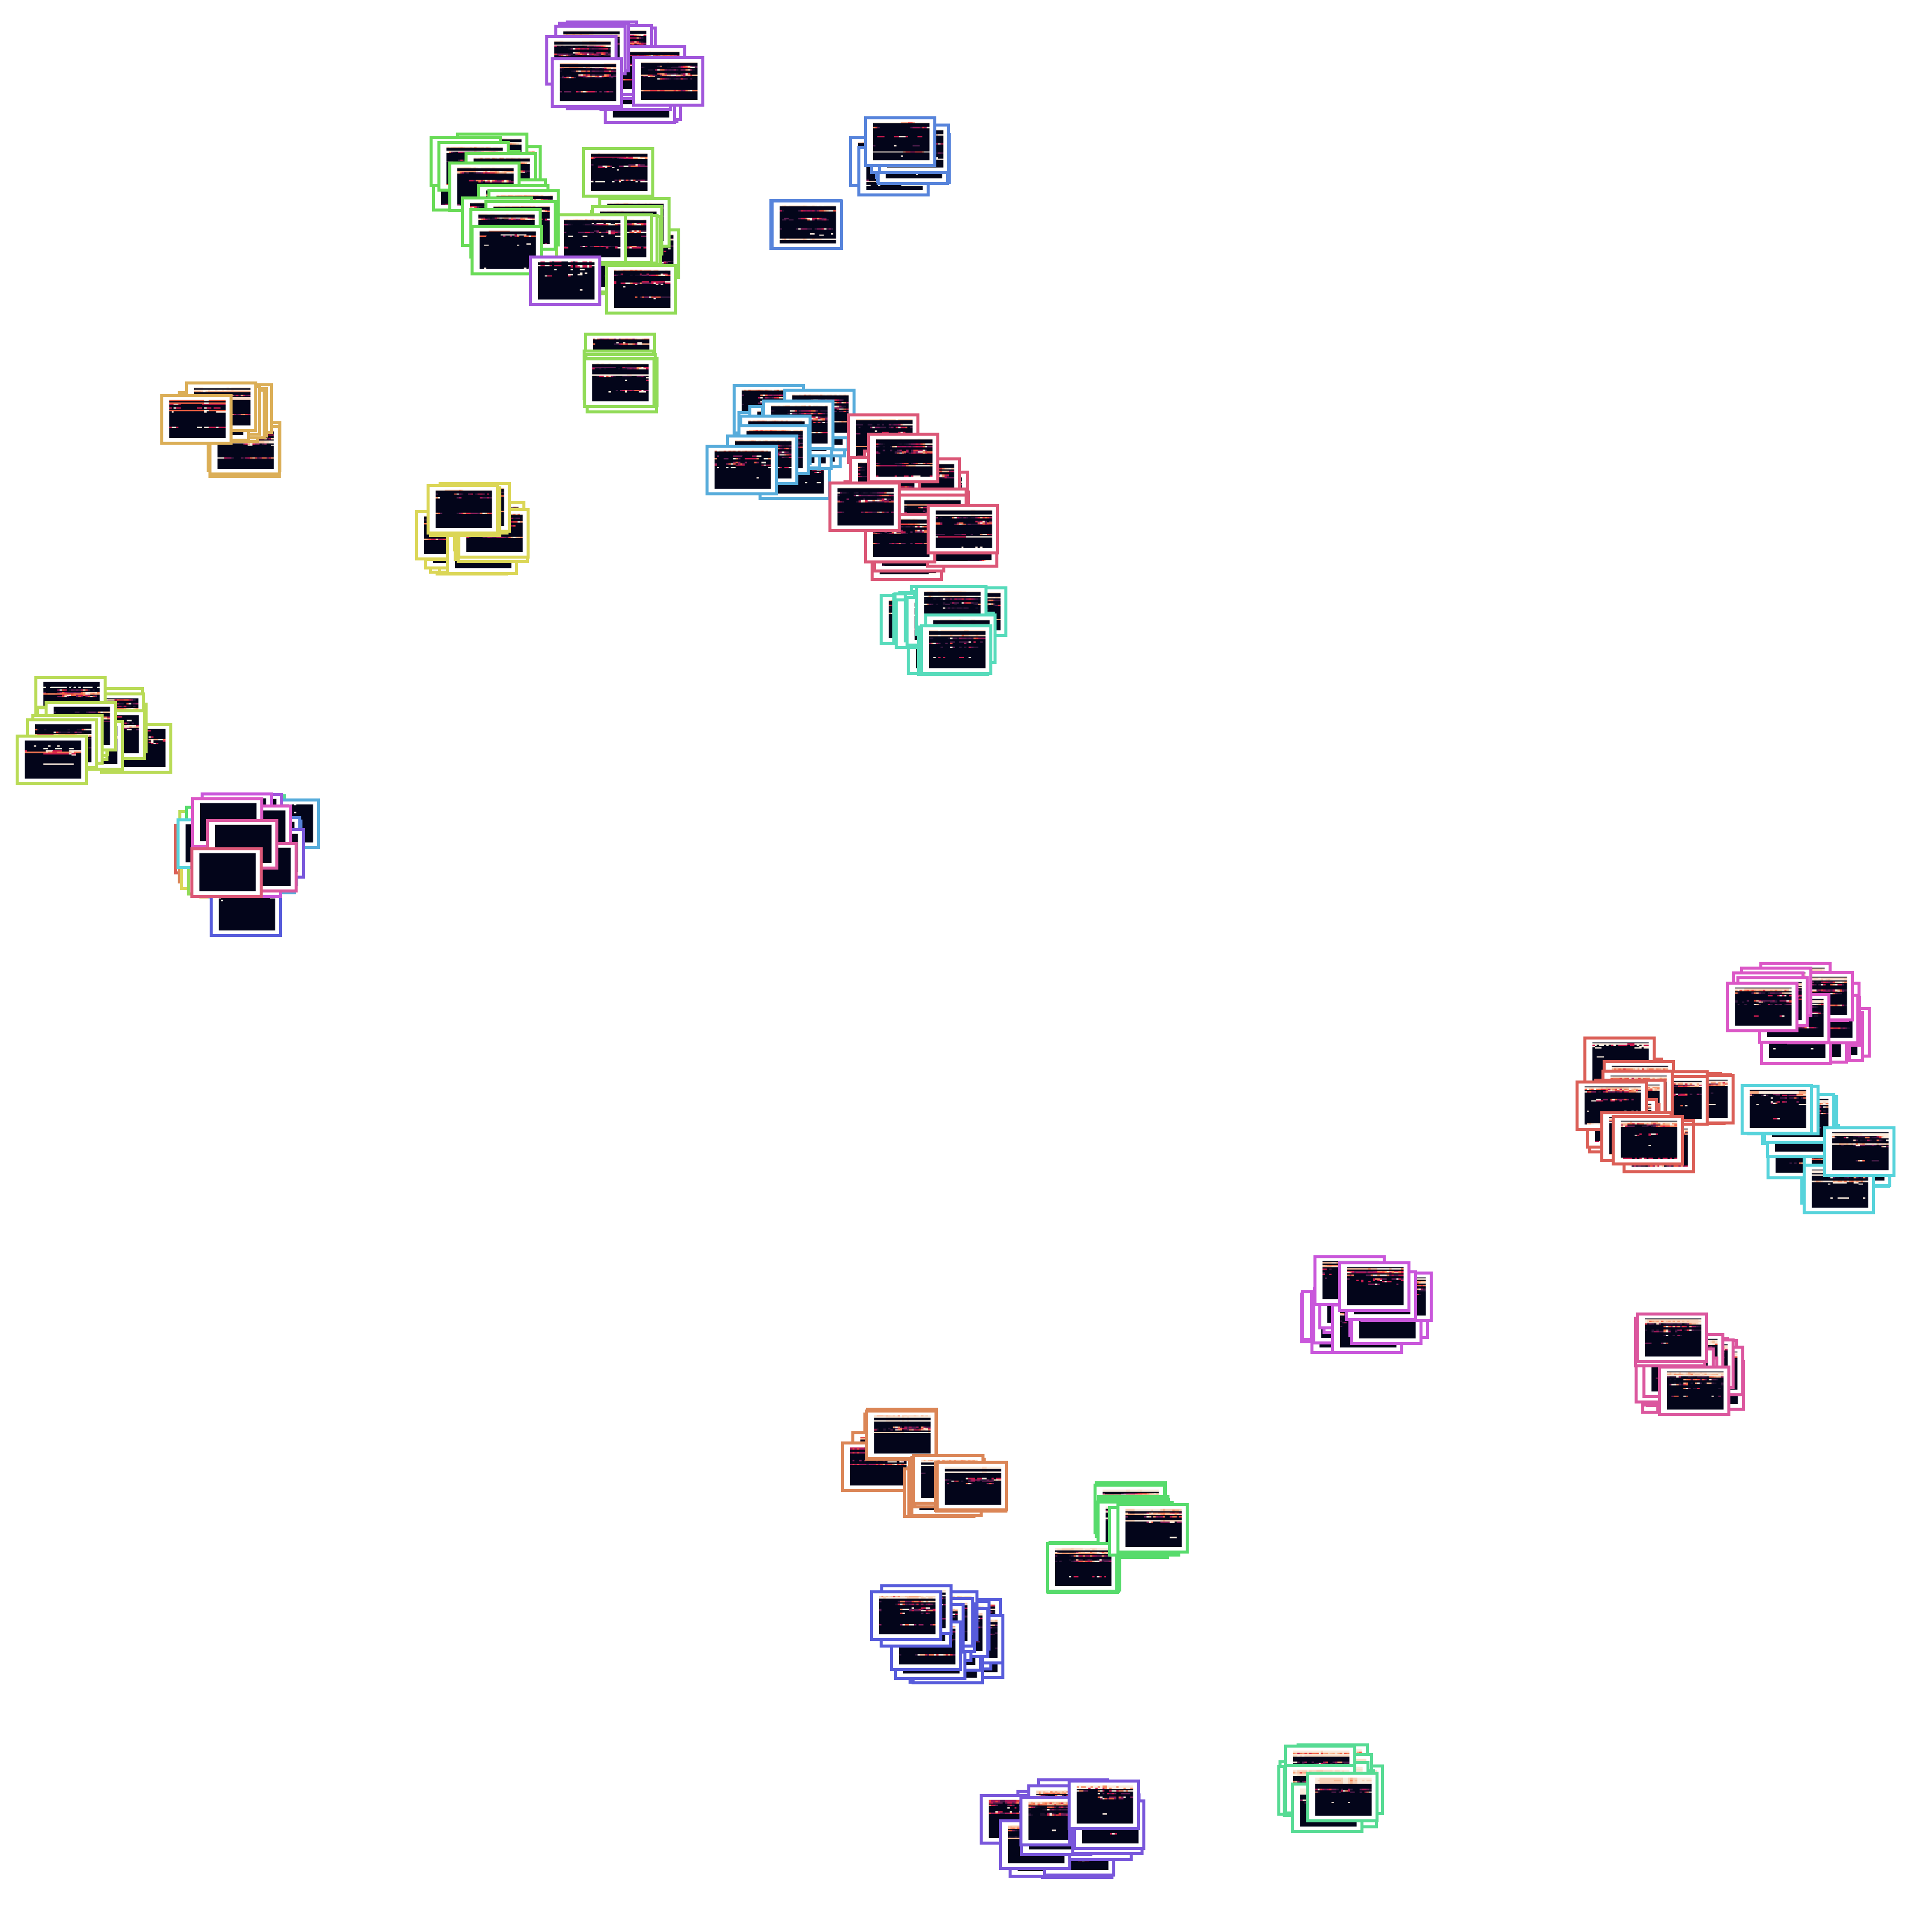
\includegraphics[width=.9\textwidth]{Figures/TSNE/TSNE_BOA/refit/img_scatter_refitall.png}
	\label{fig:tsne_boa_img_scatter_refit8}
\end{figure}